\documentclass[aspectratio=169,10pt]{beamer}

% ---------------------------------------------------------------------------
% Packages
% ---------------------------------------------------------------------------
\usepackage[utf8]{inputenc}
\usepackage[T1]{fontenc}
\usepackage{lmodern}
\usepackage{graphicx}
\usepackage{booktabs}
\usepackage{siunitx}
\usepackage{array}
\usepackage{enumitem}
\usepackage{tikz}
\usepackage{pgfplots}
\pgfplotsset{compat=1.17}
\usetikzlibrary{arrows.meta,positioning,shapes.geometric,calc}
\usepackage{multirow}
\usepackage{appendixnumberbeamer}

\sisetup{table-number-alignment = center}

% ---------------------------------------------------------------------------
% Color palette (navy / blue), same as progress deck
% ---------------------------------------------------------------------------
\definecolor{navy}{RGB}{16,32,63}
\definecolor{steel}{RGB}{43,92,157}
\definecolor{steellight}{RGB}{140,175,214}
\definecolor{bgpanel}{RGB}{240,243,247}
\definecolor{graytext}{RGB}{95,95,95}
\definecolor{municblue}{RGB}{100,140,190}
\definecolor{psuborange}{RGB}{222,164,101}
\definecolor{ppagbrown}{RGB}{150,98,58}
\definecolor{schoolgreen}{RGB}{80,165,130}
\definecolor{neutralgray}{RGB}{176,182,192}
\definecolor{statusred}{RGB}{176,36,36}
\definecolor{statuspink}{RGB}{204,100,100}
\definecolor{statuslisto}{RGB}{40,120,70}
\definecolor{placeholderbg}{RGB}{252,242,230}
\definecolor{placeholderline}{RGB}{196,120,40}
\definecolor{newdot}{RGB}{232,120,30}

% ---------------------------------------------------------------------------
% Minimalist theme
% ---------------------------------------------------------------------------
\usetheme{default}
\setbeamertemplate{navigation symbols}{}
\setbeamertemplate{headline}{}

\setbeamercolor{normal text}{fg=black,bg=white}
\setbeamercolor{structure}{fg=navy}
\setbeamercolor{title}{fg=white,bg=navy}
\setbeamercolor{frametitle}{fg=navy,bg=white}
\setbeamercolor{alerted text}{fg=steel}
\setbeamercolor{block title}{fg=white,bg=steel}
\setbeamercolor{block body}{fg=black,bg=bgpanel}
\setbeamercolor{itemize item}{fg=steel}
\setbeamercolor{itemize subitem}{fg=steellight}
\setbeamerfont{frametitle}{series=\bfseries}
\setbeamerfont{footline}{size=\scriptsize}

\setbeamertemplate{itemize item}{\raise1.2pt\hbox{\textcolor{steel}{\rule{4pt}{4pt}}}}
\setbeamertemplate{itemize subitem}{\raise1.2pt\hbox{\textcolor{steellight}{\rule{3pt}{3pt}}}}

\setlist[itemize]{itemsep=5pt, topsep=3pt, leftmargin=*}
\setlist[itemize,2]{itemsep=3pt, topsep=2pt}
\setlist[enumerate]{itemsep=5pt, topsep=3pt, leftmargin=*}

\setbeamertemplate{frametitle}{
  \vspace{0pt}
  \hspace{2pt}\textcolor{navy}{\large\bfseries\insertframetitle}\par
  \vspace{-4pt}
  \hspace{2pt}\textcolor{steel}{\rule{0.94\paperwidth}{0.7pt}}
  \vspace{-8pt}
}

\setbeamertemplate{footline}{
  \hfill
  \raisebox{6pt}{\textcolor{graytext}{\scriptsize\insertframenumber\,/\,\inserttotalframenumber}}
  \hspace{10pt}
  \vspace{6pt}
}

\setbeamertemplate{blocks}[rounded][shadow=false]

% Orange dot in the title = new slide
\newcommand{\nueva}{\textcolor{newdot}{$\bullet$}\ }
\newcommand{\fuente}[1]{\vspace{2pt}\textcolor{graytext}{\scriptsize #1}}

% One-line slide conclusion
\newcommand{\takeaway}[1]{\par\vspace{6pt}{\small\textcolor{steel}{$\Rightarrow$}\ \textbf{\textcolor{navy}{#1}}}}

% Placeholder box for pending results
\newcommand{\placeholder}[1]{%
  \begin{tikzpicture}
  \node[draw=placeholderline,thick,dashed,fill=placeholderbg,rounded corners,
        text width=0.85\textwidth,align=center,inner sep=14pt] {%
    \textcolor{placeholderline}{\Large $\varnothing$}\\[6pt]
    \textcolor{placeholderline}{\bfseries PLACEHOLDER --- results pending}\\[4pt]
    \small\textcolor{graytext} #1
  };
  \end{tikzpicture}
}

\title{Impacts of Public Early Childhood Education in Chile on Maternal Fertility and Labor Market Outcomes}
\author{Micaella Magnasco}
\date{November 2026}

\begin{document}

% =============================================================================
% 1. TITLE
% =============================================================================
\begin{frame}[plain]
\vspace{40pt}
\begin{center}
{\LARGE\bfseries\color{navy} Impacts of Public Early Childhood Education\\[3pt] in Chile on Maternal Fertility\\[3pt] and Labor Market Outcomes}

\vspace{8pt}
{\large\color{graytext} Short-run effects --- progress update}

\vspace{10pt}
\textcolor{steel}{\rule{0.5\paperwidth}{0.6pt}}

\vspace{18pt}
{\normalsize
Andr\'es Hojman \quad Marigen Narea \quad Jorge Rodr\'iguez \quad Pedro Carneiro \quad Micaella Magnasco\\[8pt]
\small Pontificia Universidad Cat\'olica de Chile \\[2pt]
\small November 2026
}
\end{center}
\end{frame}

% =============================================================================
% AGENDA
% =============================================================================
\begin{frame}{Reminder and plan for today}
\begin{block}{Question}
\small What are the effects of the public expansion of early childhood education in Chile on mothers' labor market participation and fertility?
\end{block}
\vspace{4pt}
\begin{columns}[T]
\begin{column}{0.56\textwidth}
{\small\textcolor{steel}{\textbf{Design}}}
\begin{itemize}
  \footnotesize
  \item Staggered difference-in-differences with event study
  \item \textbf{Treatment}: the UV, the year it opens its first public preschool
  \item \textbf{Control}: UVs that never get one
  \item \textbf{Panel}: UV $\times$ year, with UV and year fixed effects; woman fixed effects as a check
  \item \textbf{Effect}: intent-to-treat of access, not individual take-up
\end{itemize}
\end{column}
\begin{column}{0.40\textwidth}
{\small\textcolor{steel}{\textbf{Today}}}
\begin{itemize}
  \footnotesize
  \item \textbf{Sample changes}: who enters and leaves, and why
  \item \textbf{Data fixes}: recap and the UV crosswalk
  \item \textbf{Results}, one by one: first stage, formal employment, earnings, fertility
  \item \textbf{What is pending} from our conversations
\end{itemize}
\end{column}
\end{columns}
\end{frame}

% =============================================================================
% SAMPLE CHANGES
% =============================================================================
\begin{frame}{What changed in the samples}
\begin{columns}[T]
\begin{column}{0.35\textwidth}
{\small\textcolor{steel}{\textbf{Labor market}}}
\begin{itemize}
  \footnotesize
  \item \textbf{Who}: vulnerable, with a child $<$5 in at least one year, 2014--2024
  \item \textbf{Enters}: first year in the data, even before her first child \\ \textcolor{graytext}{Before: first year with a child $<$5}
  \item \textbf{Leaves}: not because of age, within the 18--70 panel \\ \textcolor{graytext}{Before: years after 49 without a child $<$5 were dropped}
  \item \textbf{New}: balanced version, all 11 years
\end{itemize}
\end{column}
\begin{column}{0.32\textwidth}
{\small\textcolor{steel}{\textbf{Fertility}}}
\begin{itemize}
  \footnotesize
  \item \textbf{Who}: vulnerable, aged 18--35 in 2014, with or without children \\ \textcolor{graytext}{Before: 18--49 each year}
  \item \textbf{Enters}: first year in the data
  \item \textbf{Leaves}: never because of age
  \item \textbf{New}: balanced version, all 11 years
\end{itemize}
\end{column}
\begin{column}{0.29\textwidth}
{\small\textcolor{steel}{\textbf{Why}}}
\begin{itemize}
  \footnotesize
  \item Keep changes in who is observed out of the effects
  \item Bring the panel as close to balanced as possible
  \item Compare women at the same stage of motherhood
  \item Women 18--35 in 2014 have 80\% of births, and no one enters or leaves by turning 18 or 50
\end{itemize}
\end{column}
\end{columns}
\takeaway{We follow the same women for longer, so composition weighs less on the estimates.}
\end{frame}

\begin{frame}{Who is in each sample}
\begin{columns}[T]
\begin{column}{0.31\textwidth}
{\small\textcolor{steel}{\textbf{First stage}}}
\begin{itemize}
  \footnotesize
  \item Children aged 0--4 of vulnerable mothers
  \item Only years at those ages, if the mother is observed that year
\end{itemize}
\end{column}
\begin{column}{0.33\textwidth}
{\small\textcolor{steel}{\textbf{Labor market}}}
\begin{itemize}
  \footnotesize
  \item Defined by \textbf{being a mother}, at any age
  \item \textbf{817k mothers}
\end{itemize}
\end{column}
\begin{column}{0.33\textwidth}
{\small\textcolor{steel}{\textbf{Fertility}}}
\begin{itemize}
  \footnotesize
  \item Defined by \textbf{age}, with or without children
  \item \textbf{1.02M women}
\end{itemize}
\end{column}
\end{columns}

\vspace{6pt}
\colorbox{bgpanel}{\parbox{0.97\linewidth}{\raggedright\footnotesize
\textbf{In every sample}: women aged 18--70 in the FPS/RSH, 2014--2024; vulnerable = 60\% most vulnerable, fixed the first year she is classified. A woman has data only in years she is in the registry with a valid UV. Years 2014--2015 count only if she is also in 2016, and use her 2016 UV. Only UVs without a preschool in 2014: 319 treated, 4,174 never treated.}}
\takeaway{The labor sample follows mothers; the fertility sample follows women of a fixed age group.}
\end{frame}

% =============================================================================
% DATA FIXES
% =============================================================================
\begin{frame}{Data fixes: recap}
\begin{columns}[c]
\begin{column}{0.50\textwidth}
\centering
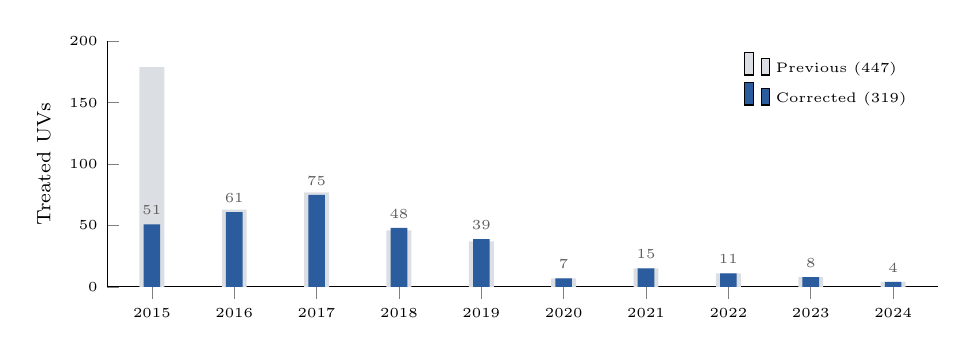
\begin{tikzpicture}
\begin{axis}[
  ybar,
  bar width=9pt,
  width=\linewidth,
  height=4.7cm,
  symbolic x coords={2015,2016,2017,2018,2019,2020,2021,2022,2023,2024},
  xtick=data,
  ymin=0, ymax=200,
  ylabel={Treated UVs},
  ylabel style={font=\scriptsize},
  tick label style={font=\tiny},
  axis lines*=left,
  enlarge x limits=0.06,
  legend style={font=\tiny,draw=none,at={(0.98,0.98)},anchor=north east},
  legend cell align=left,
]
\addplot[fill=neutralgray!45,draw=none,bar shift=0pt] coordinates {(2015,179)(2016,63)(2017,77)(2018,46)(2019,37)(2020,7)(2021,15)(2022,11)(2023,8)(2024,4)};
\addplot[fill=steel,draw=none,bar shift=0pt,bar width=6pt,nodes near coords,nodes near coords style={font=\tiny,text=graytext}] coordinates {(2015,51)(2016,61)(2017,75)(2018,48)(2019,39)(2020,7)(2021,15)(2022,11)(2023,8)(2024,4)};
\legend{Previous (447),Corrected (319)}
\end{axis}
\end{tikzpicture}
\end{column}
\begin{column}{0.46\textwidth}
\begin{itemize}
  \small
  \item \textbf{Opening years}
  \begin{itemize}
    \footnotesize
    \item Most 2015 ``openings'' were centers already operating
    \item Treated UVs: \textbf{447 $\to$ 319}
  \end{itemize}
  \item \textbf{Earnings}
  \begin{itemize}
    \footnotesize
    \item Before: only taxable (dependent) income if she had any
    \item Now: taxable + independent income
  \end{itemize}
  \item \textbf{UV crosswalk}
  \begin{itemize}
    \footnotesize
    \item Fixed again this week (next slide)
  \end{itemize}
\end{itemize}
\end{column}
\end{columns}
\takeaway{These fixes correct who is treated and how earnings are measured.}
\end{frame}

\begin{frame}{UV crosswalk: one rule for all years}
\centering
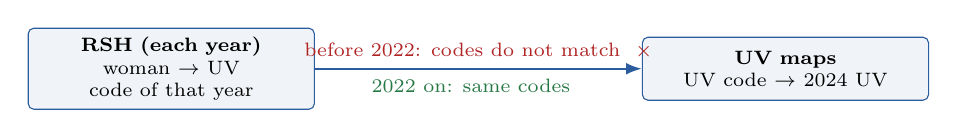
\begin{tikzpicture}[
  src/.style={draw=steel,fill=bgpanel,rounded corners=2pt,align=center,font=\scriptsize,minimum height=0.8cm,text width=3.4cm}]
\node[src] (rsh) at (-3.9,0) {\textbf{RSH (each year)}\\woman $\to$ UV code of that year};
\node[src] (map) at (3.9,0) {\textbf{UV maps}\\UV code $\to$ 2024 UV};
\draw[-{Latex[length=2mm]},thick,steel] (rsh) -- (map)
  node[midway,above,font=\scriptsize,text=statusred] {before 2022: codes do not match \ $\times$}
  node[midway,below,font=\scriptsize,text=statuslisto] {2022 on: same codes \ $\checkmark$};
\end{tikzpicture}

\vspace{6pt}
\raggedright
\begin{columns}[T]
\begin{column}{0.46\textwidth}
\begin{itemize}
  \small
  \item \textbf{So before 2022}, we follow where each code's households live the next year
  \item \textbf{Before}: UV codes treated differently by quality $\to$ the problem spread to more years
  \item \textbf{Now}: every code follows the same rule, for all years
\end{itemize}
\end{column}
\begin{column}{0.50\textwidth}
\begin{center}
\footnotesize
\begin{tabular}{@{}lcc@{}}
\toprule
 & Before & Now \\
\midrule
Women changing UV per year & 19--26\% & \textbf{4--9\%} \\
Of those, with the same RSH code & 50--75\% & \textbf{0--1\%} \\
Treated UVs with data from 2014 & 241 & \textbf{299} \\
First stage, $k=-2$ & +0.9pp & \textbf{+0.3pp} \\
\bottomrule
\end{tabular}
\end{center}
\end{column}
\end{columns}
\takeaway{The crosswalk improved: spurious moves are gone and the pre-trend in the first stage is smaller.}
\end{frame}

\begin{frame}{UV crosswalk: the 2022 jump remains}
\begin{columns}[T]
\begin{column}{0.50\textwidth}
{\small\textcolor{steel}{\textbf{What we see}}}
\begin{itemize}
  \footnotesize
  \item Women changing UV in 2022: \textbf{23\%}, vs.\ 4--9\% other years
  \item Cartography and method change that year
  \item Sample UVs added in 2022: \textbf{203 control, 12 treated}, vs.\ 0--30 other years
  \item Could mean 15--18\% of women have another UV in 2016--2021 (inferred, not measured)
\end{itemize}
\end{column}
\begin{column}{0.46\textwidth}
{\small\textcolor{steel}{\textbf{So far}}}
\begin{itemize}
  \footnotesize
  \item Similar in both groups: \textbf{25.9\% treated, 26.3\% control}
  \item Raw levels: \textbf{the treated $-$ control gap does not jump in 2022}
\end{itemize}
\vspace{2pt}
{\small\textcolor{steel}{\textbf{Next}}}
\begin{itemize}
  \footnotesize
  \item Woman FE with the UV fixed from 2022
  \item Without 2021 codes split across UVs
\end{itemize}
\end{column}
\end{columns}
\takeaway{In raw levels, results do not seem driven by 2022, but this jump needs a deeper look.}
\end{frame}

% =============================================================================
% FIRST STAGE
% =============================================================================
\begin{frame}{First stage: enrollment rises the year a preschool opens}
\begin{columns}[c]
\begin{column}{0.58\textwidth}
\centering
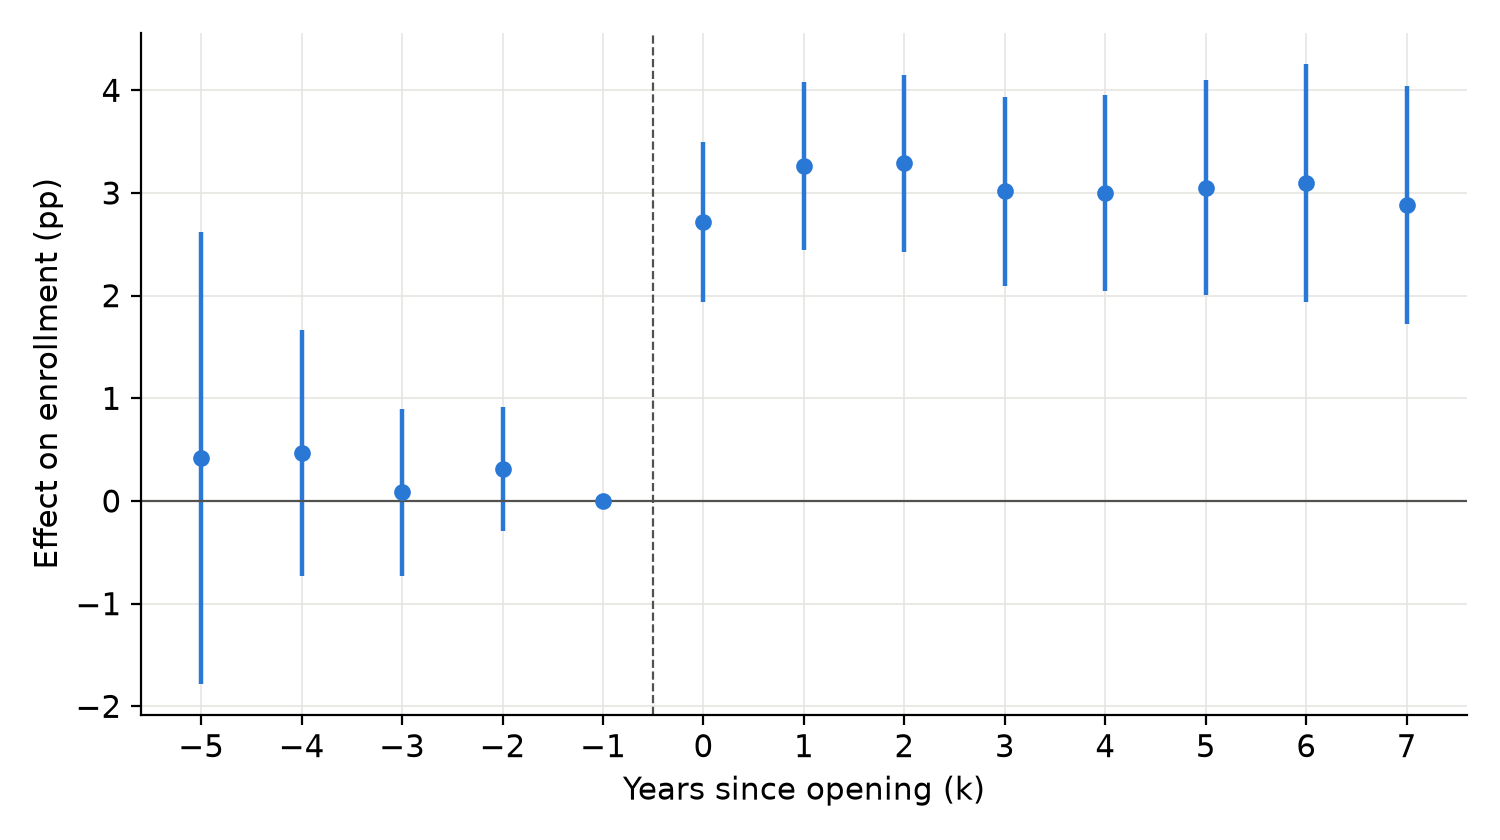
\includegraphics[width=\linewidth,height=0.62\textheight,keepaspectratio]{../RIS/20261104/graficos/en_pe.png}
\end{column}
\begin{column}{0.40\textwidth}
\begin{itemize}
  \footnotesize
  \item \textbf{Measure}: share of children 0--4 of vulnerable mothers enrolled
  \item \textbf{Year before opening}: treated 31.7\%, control 33.0\%
  \item \textbf{Pre-trends}: none ($p=0.81$)
  \item \textbf{Estimate}, first 8 years: \textbf{+3.0pp}, significant, $\approx$3.6 more children per UV
  \item \textbf{Last meeting}: +3.6pp, with a significant $k=-2$ that is now gone
\end{itemize}
\end{column}
\end{columns}
\takeaway{Enrollment jumps when the first preschool opens and stays higher: from 34\% to 37\%, about 3.6 more children per UV.}
\par\fuente{Sun--Abraham, weighted, 95\% CI clustered by UV, ref.\ $k=-1$. Levels: control mean.}
\end{frame}

% =============================================================================
% EMPLOYMENT
% =============================================================================
\begin{frame}{Labor market results: who we measure}
\vspace{4pt}
{\small \textbf{Vulnerable mothers}: a child $<$5 in at least one year, 2014--2024, at any age.}
\vspace{6pt}
\begin{columns}[T]
\begin{column}{0.48\textwidth}
{\small\textcolor{steel}{\textbf{Full sample}}: \textbf{817k mothers}}
\begin{itemize}
  \footnotesize
  \item Counts in the UV where she lives that year
  \item Not counted in years in a UV with a preschool in 2014
\end{itemize}
\vspace{4pt}
{\small\textcolor{steel}{\textbf{Woman FE}}: \textbf{5.6M mother-years}}
\begin{itemize}
  \footnotesize
  \item Compared with herself, in the first valid UV where she appears, even if she moves
  \item Treated UV: she must appear before the opening. Control UV: any year
\end{itemize}
\end{column}
\begin{column}{0.48\textwidth}
{\small\textcolor{steel}{\textbf{Balanced}}: \textbf{247k mothers}}
\begin{itemize}
  \footnotesize
  \item Same, only women with all 11 years in these UVs
\end{itemize}
\vspace{24pt}
{\small\textcolor{steel}{\textbf{Woman FE, balanced}}: \textbf{357k mothers}}
\begin{itemize}
  \footnotesize
  \item Same, only women who appear in 2014 and have all 11 years, in any UV
\end{itemize}
\end{column}
\end{columns}
\takeaway{The same mothers, measured four ways: from the UV where they live to each mother against herself.}
\end{frame}

\begin{frame}{Employment: more mothers enter formal work, gradually}
\begin{columns}[c]
\begin{column}{0.58\textwidth}
\centering
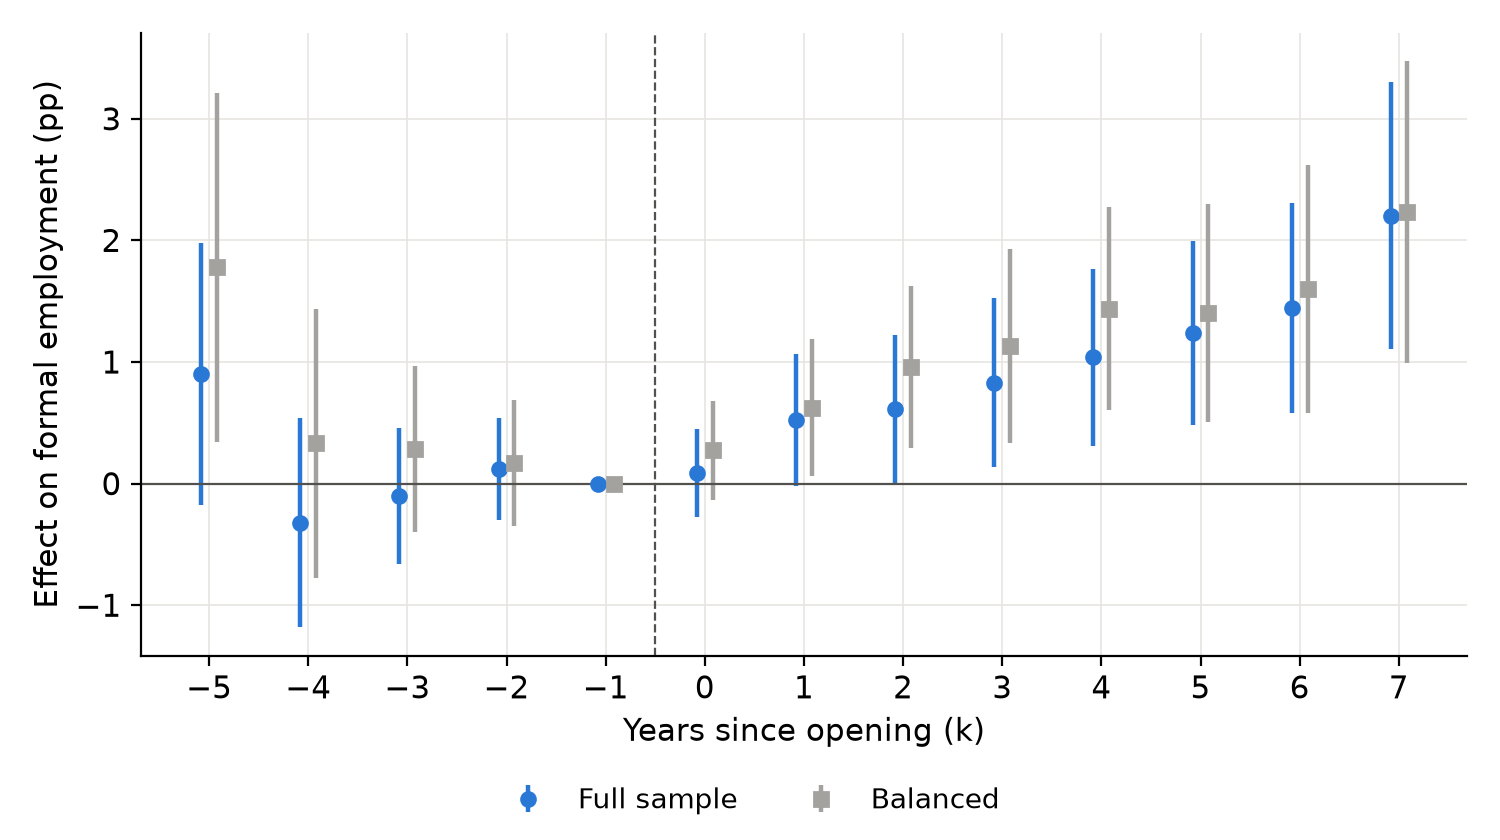
\includegraphics[width=\linewidth,height=0.62\textheight,keepaspectratio]{../RIS/20261104/graficos/en_empleo.png}
\end{column}
\begin{column}{0.40\textwidth}
\begin{itemize}
  \footnotesize
  \item \textbf{Measure}: share of mothers with formal earnings in the year
  \item \textbf{Year before opening}: 54.8\% in both groups
  \item \textbf{Pre-trends}: none ($p=0.15$, balanced $p=0.18$)
  \item \textbf{Estimate}, first 8 years: \textbf{+1.0pp} full, \textbf{+1.2pp} balanced, both significant
  \item $\approx$2.5 more working mothers per UV
  \item \textbf{Last meeting}: +1.5pp, with negative pre-trend coefficients that are now around zero
\end{itemize}
\end{column}
\end{columns}
\takeaway{When the first preschool opens, formal employment rises gradually: from 54.6\% to 55.6\% of mothers.}
\par\fuente{Sun--Abraham, weighted, 95\% CI clustered by UV, ref.\ $k=-1$. Levels: control mean.}
\end{frame}

\begin{frame}{Employment, woman fixed effects: also rises gradually}
\begin{columns}[c]
\begin{column}{0.58\textwidth}
\centering
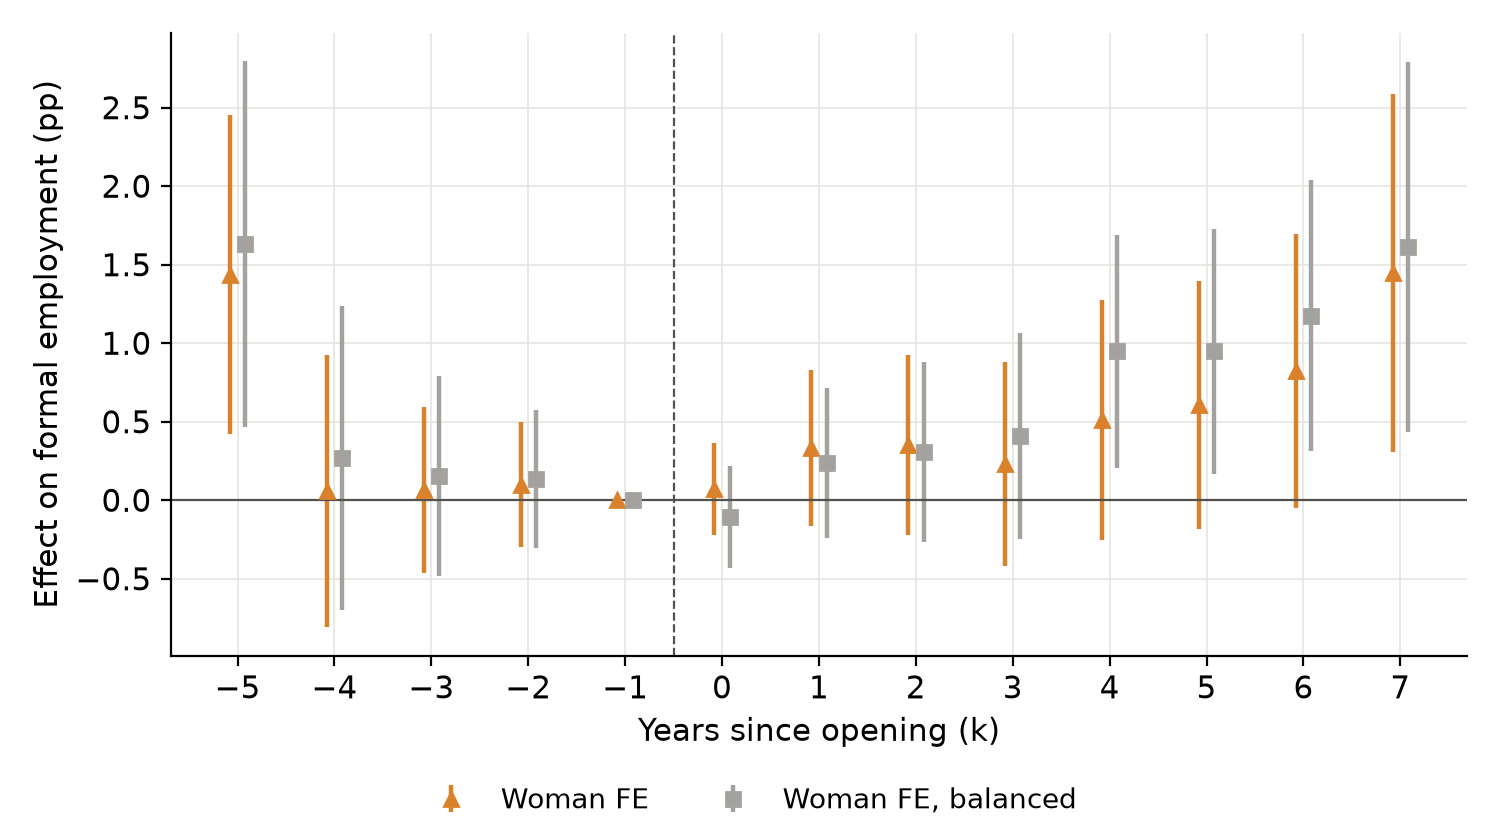
\includegraphics[width=\linewidth,height=0.62\textheight,keepaspectratio]{../RIS/20261104/graficos/en_empleo_ef.png}
\end{column}
\begin{column}{0.40\textwidth}
\begin{itemize}
  \footnotesize
  \item \textbf{Measure}: whether each mother has formal earnings in the year
  \item \textbf{Woman fixed effects}: each mother compared with herself, assigned to the first UV where she appears
  \item \textbf{Start}: $\approx$55\% of these mothers have formal earnings
  \item \textbf{Pre-trends}: none ($p=0.06$, balanced $p=0.10$)
  \item \textbf{Estimate}, first 8 years: their share rises \textbf{+0.55pp}, \textbf{+0.7pp} balanced (significant)
\end{itemize}
\end{column}
\end{columns}
\takeaway{Following the same women, the share of mothers with formal earnings also rises gradually, at about half the size: from 54.7\% to 55.3\%.}
\par\fuente{Sun--Abraham, 95\% CI, ref.\ $k=-1$. Levels: control mean.}
\end{frame}

% =============================================================================
% EARNINGS
% =============================================================================
\begin{frame}{Earnings including zeros rise gradually}
\begin{columns}[c]
\begin{column}{0.58\textwidth}
\centering
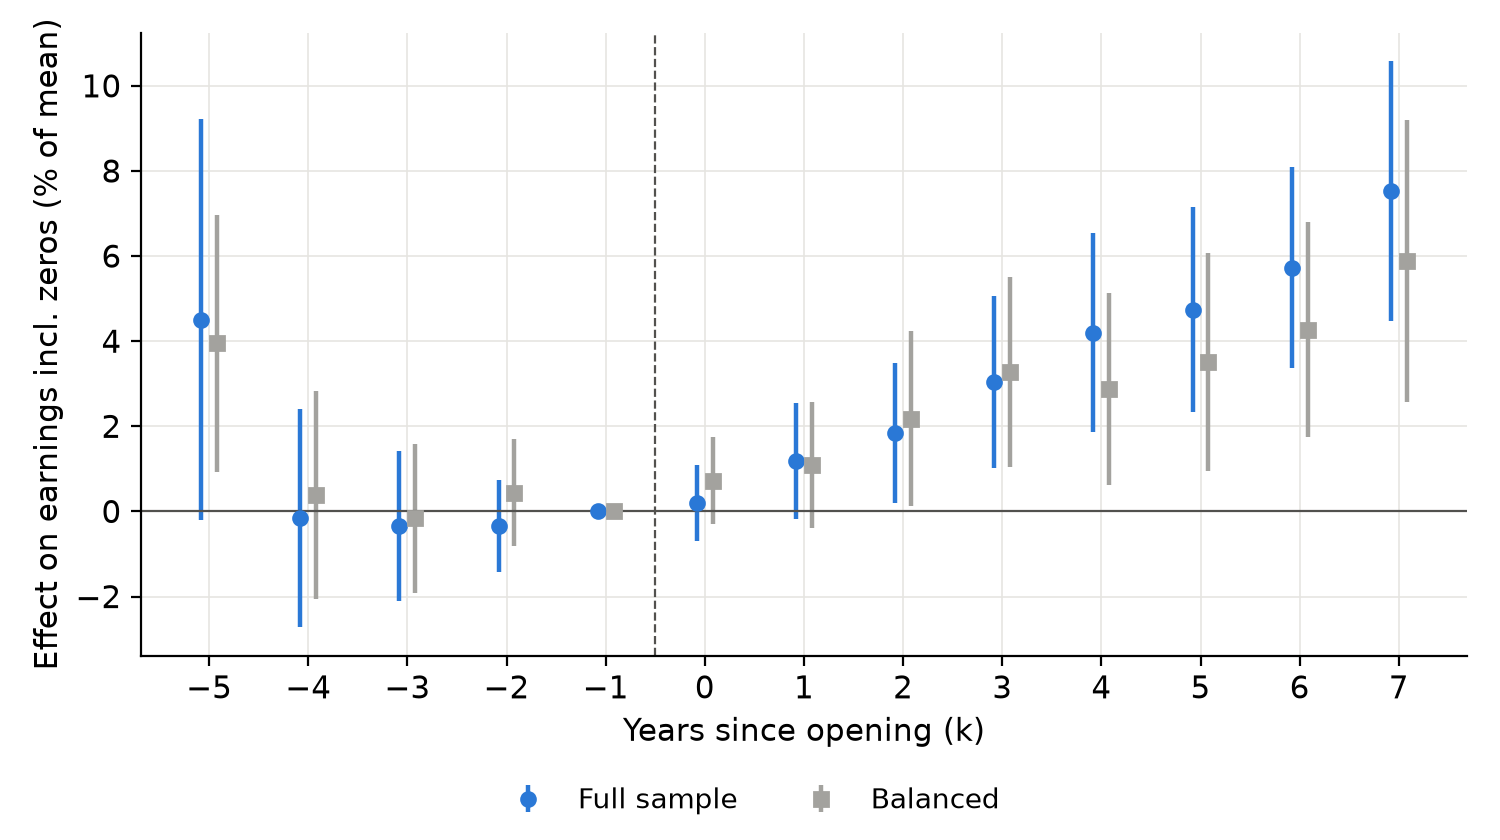
\includegraphics[width=\linewidth,height=0.62\textheight,keepaspectratio]{../RIS/20261104/graficos/en_ingreso.png}
\end{column}
\begin{column}{0.40\textwidth}
\begin{itemize}
  \footnotesize
  \item \textbf{Measure}: formal earnings of all mothers, zero if none, relative to the year's mean
  \item \textbf{Level}, 2024 pesos: $\approx$CLP 260k a month in 2014, $\approx$CLP 424k in 2024; about half have no formal earnings
  \item \textbf{Pre-trends}: none in full ($p=0.13$), yes in balanced ($p=0.04$)
  \item \textbf{Estimate}, first 8 years: \textbf{+3.6\%} full, \textbf{+3.0\%} balanced, both significant
  \item \textbf{Last meeting}: +4.4\%
\end{itemize}
\end{column}
\end{columns}
\takeaway{Mothers' average earnings in the UV rise gradually: from about CLP 335k to 347k a month, in 2024 pesos.}
\par\fuente{Sun--Abraham, weighted, 95\% CI clustered by UV, ref.\ $k=-1$. Levels: mean 2016--2024, approximate.}
\end{frame}

\begin{frame}{Earnings including zeros, woman fixed effects}
\begin{columns}[c]
\begin{column}{0.58\textwidth}
\centering
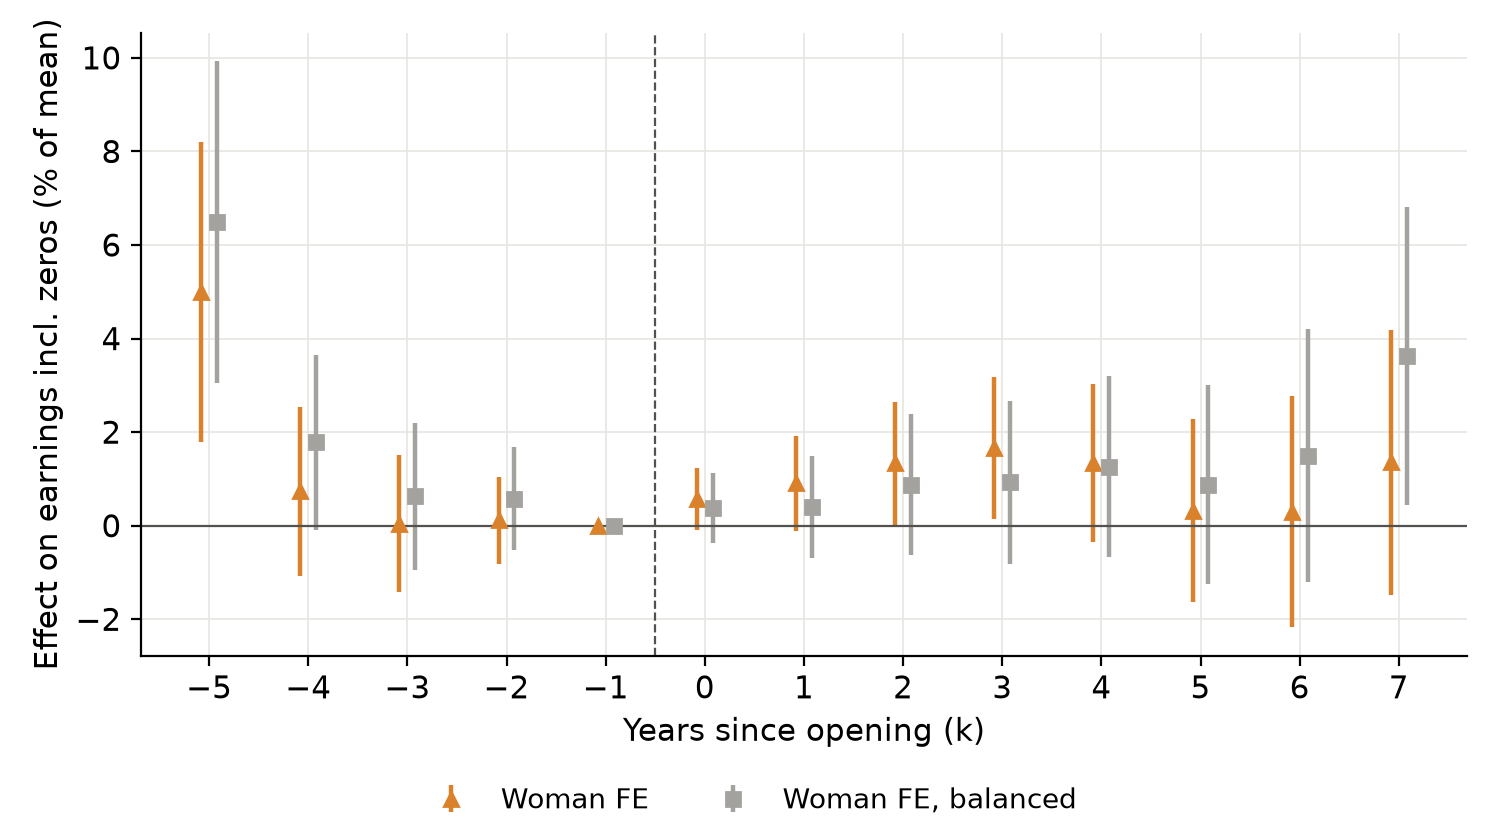
\includegraphics[width=\linewidth,height=0.62\textheight,keepaspectratio]{../RIS/20261104/graficos/en_ingreso_ef.png}
\end{column}
\begin{column}{0.40\textwidth}
\begin{itemize}
  \footnotesize
  \item \textbf{Woman fixed effects}: each mother compared with herself, in the first UV where she appears
  \item \textbf{Level}, 2024 pesos: $\approx$CLP 260k a month in 2014, $\approx$CLP 424k in 2024
  \item \textbf{Pre-trends}: yes ($p=0.02$, balanced $p<0.01$)
  \item \textbf{Estimate}, first 8 years: \textbf{+1.0\%}, \textbf{+1.2\%} balanced, not significant
\end{itemize}
\end{column}
\end{columns}
\takeaway{With woman fixed effects, the rise is small and not significant: about CLP 3k a month, smaller than in the UV.}
\par\fuente{Sun--Abraham, 95\% CI, ref.\ $k=-1$. Levels: mean 2016--2024, approximate.}
\end{frame}

\begin{frame}{Earnings of mothers with earnings}
\begin{columns}[c]
\begin{column}{0.58\textwidth}
\centering
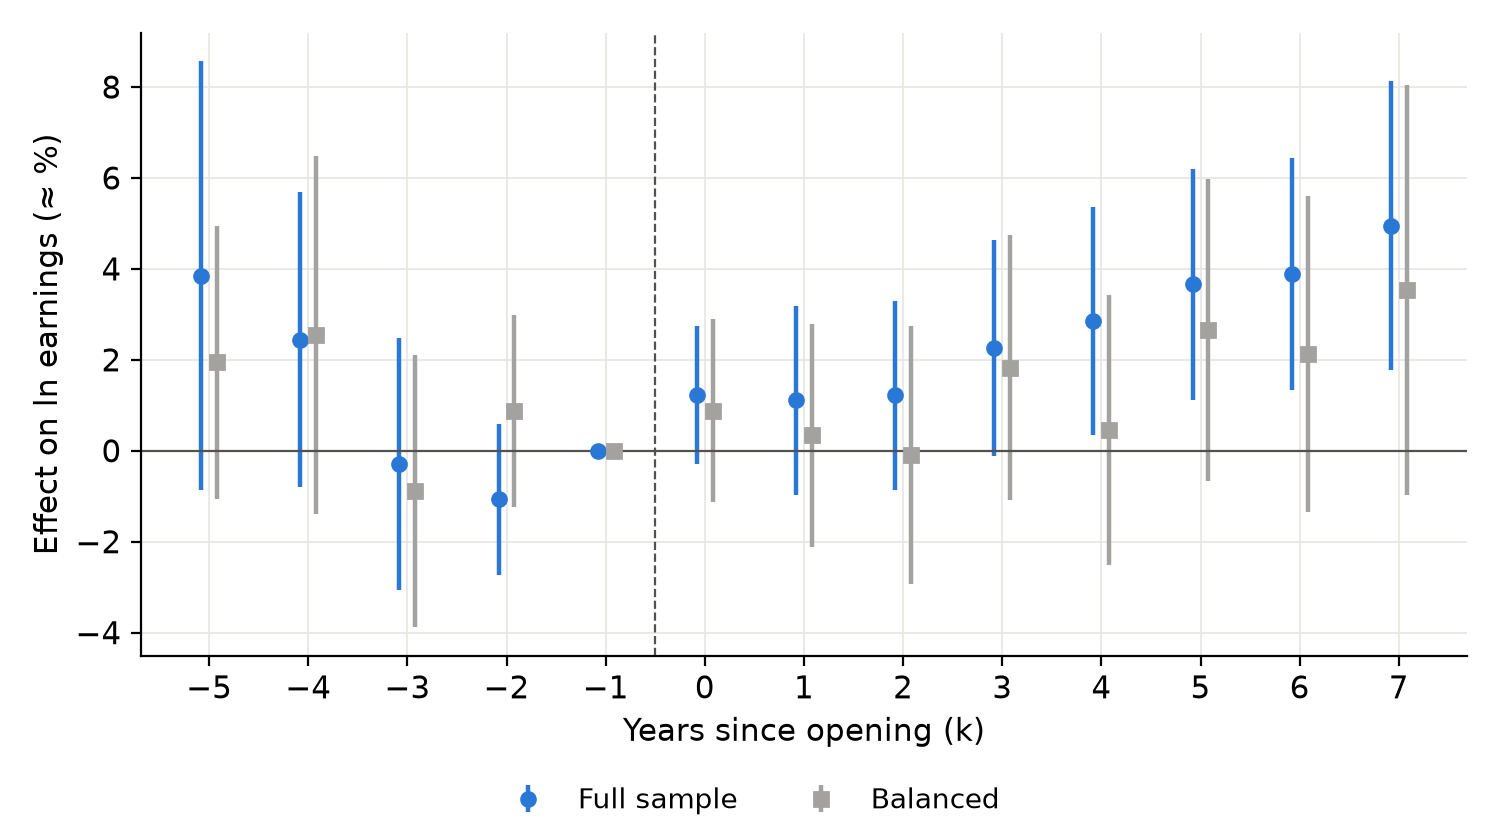
\includegraphics[width=\linewidth,height=0.62\textheight,keepaspectratio]{../RIS/20261104/graficos/en_ln.png}
\end{column}
\begin{column}{0.40\textwidth}
\begin{itemize}
  \footnotesize
  \item \textbf{Measure}: ln annual earnings, only mothers with formal earnings that year
  \item \textbf{Level}, 2024 pesos: $\approx$CLP 470k a month in 2014, $\approx$CLP 770k in 2024
  \item \textbf{Pre-trends}: none ($p=0.20$, balanced $p=0.20$)
  \item \textbf{Estimate}, first 8 years: \textbf{+2.65\%} full, significant; \textbf{+1.5\%} balanced, not significant
  \item Annual: mixes wages and months worked; who has earnings can change
\end{itemize}
\end{column}
\end{columns}
\takeaway{Earnings of mothers with earnings rise about CLP 17k a month in the UV.}
\par\fuente{Sun--Abraham, weighted, 95\% CI clustered by UV, ref.\ $k=-1$. Levels: mean 2016--2024, approximate.}
\end{frame}

\begin{frame}{Earnings of mothers with earnings, woman fixed effects}
\begin{columns}[c]
\begin{column}{0.58\textwidth}
\centering
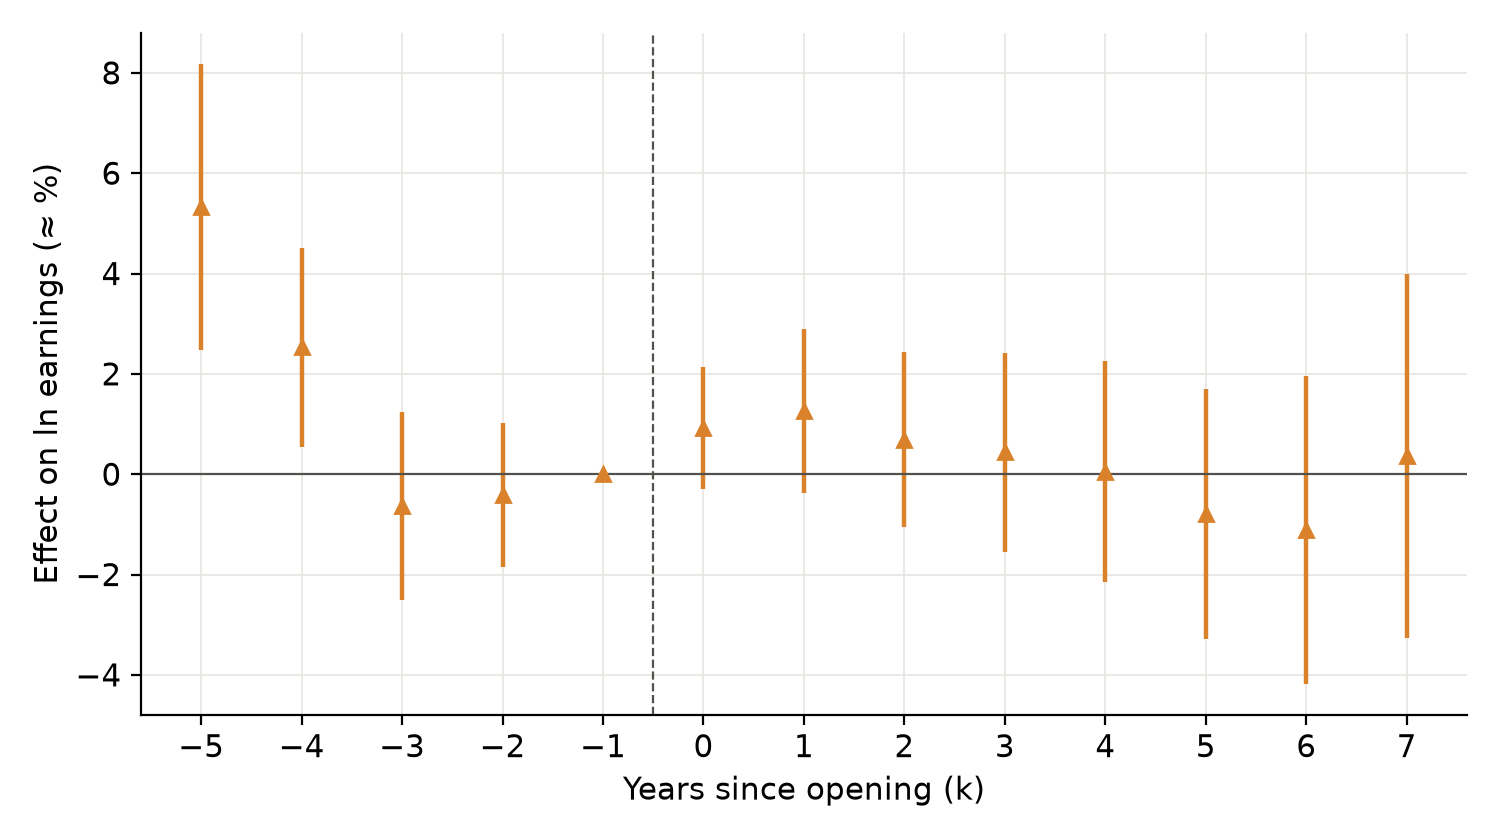
\includegraphics[width=\linewidth,height=0.62\textheight,keepaspectratio]{../RIS/20261104/graficos/en_ln_ef.png}
\end{column}
\begin{column}{0.40\textwidth}
\begin{itemize}
  \footnotesize
  \item \textbf{Woman fixed effects}: each mother compared with herself, only years with formal earnings
  \item \textbf{Level}, 2024 pesos: $\approx$CLP 470k a month in 2014, $\approx$CLP 770k in 2024
  \item \textbf{Pre-trends}: yes ($p<0.01$)
  \item \textbf{Estimate}, first 8 years: \textbf{+0.2\%}, not significant
  \item Women who start working after the opening have no earlier year to compare, so their entry into work is not captured
\end{itemize}
\end{column}
\end{columns}
\takeaway{With woman fixed effects we do not see earnings rise; with these pre-trends, it is the least reliable version.}
\par\fuente{Sun--Abraham, 95\% CI, ref.\ $k=-1$.}
\end{frame}

\begin{frame}{How much of the earnings rise comes from more mothers working?}
\begin{itemize}
  \footnotesize
  \item Average earnings can rise because \textbf{more mothers work} or because \textbf{those who work earn more}
  \item If only more mothers worked, each earning the mean (CLP 630k): +1pp is 1 more mother in 100, so the average rises by \textbf{CLP 6.3k}
\end{itemize}
\vspace{4pt}
\begin{center}
\scriptsize
\setlength{\tabcolsep}{6pt}
\begin{tabular}{@{}lcccc@{}}
\toprule
First 8 years, 2024 pesos & More employment & Rise from employment alone & Actual rise & Share explained \\
\midrule
Full sample & +1.0pp & CLP 6.3k & CLP 12k & $\approx$half \\
Balanced & +1.2pp & CLP 7.6k & CLP 10k & $\approx$three quarters \\
Woman FE & +0.55pp & CLP 3.5k & CLP 3.2k & $\approx$all \\
Woman FE, balanced & +0.7pp & CLP 4.3k & CLP 4.1k & $\approx$all \\
\bottomrule
\end{tabular}
\end{center}
\takeaway{More mothers working explains about half of the rise in the UV, and about all of it with woman fixed effects. The rest in the UV would come from mothers already working or from who lives there.}
\par\fuente{Approximate: new workers assumed to earn mean earnings.}
\end{frame}

% =============================================================================
% FERTILITY
% =============================================================================
\begin{frame}{Fertility results: who we measure}
\vspace{4pt}
{\small \textbf{Vulnerable women aged 18--35 in 2014}, with or without children.}
\vspace{6pt}
\begin{columns}[T]
\begin{column}{0.48\textwidth}
{\small\textcolor{steel}{\textbf{Full sample}}: \textbf{1.02M women}}
\begin{itemize}
  \footnotesize
  \item Counts in the UV where she lives that year
  \item Not counted in years in a UV with a preschool in 2014
\end{itemize}
\vspace{4pt}
{\small\textcolor{steel}{\textbf{Woman FE}}: \textbf{6.9M woman-years}}
\begin{itemize}
  \footnotesize
  \item Compared with herself, in the first valid UV where she appears, even if she moves
  \item Treated UV: she must appear before the opening. Control UV: any year
\end{itemize}
\end{column}
\begin{column}{0.48\textwidth}
{\small\textcolor{steel}{\textbf{Balanced}}: \textbf{302k women}}
\begin{itemize}
  \footnotesize
  \item Same, only women with all 11 years in these UVs
\end{itemize}
\vspace{24pt}
{\small\textcolor{steel}{\textbf{Woman FE, balanced}}: \textbf{431k women}}
\begin{itemize}
  \footnotesize
  \item Same, only women who appear in 2014 and have all 11 years, in any UV
\end{itemize}
\end{column}
\end{columns}
\takeaway{The same four versions, now for women of a fixed age group.}
\end{frame}

\begin{frame}{Births fall sharply, in treated and control alike}
\centering
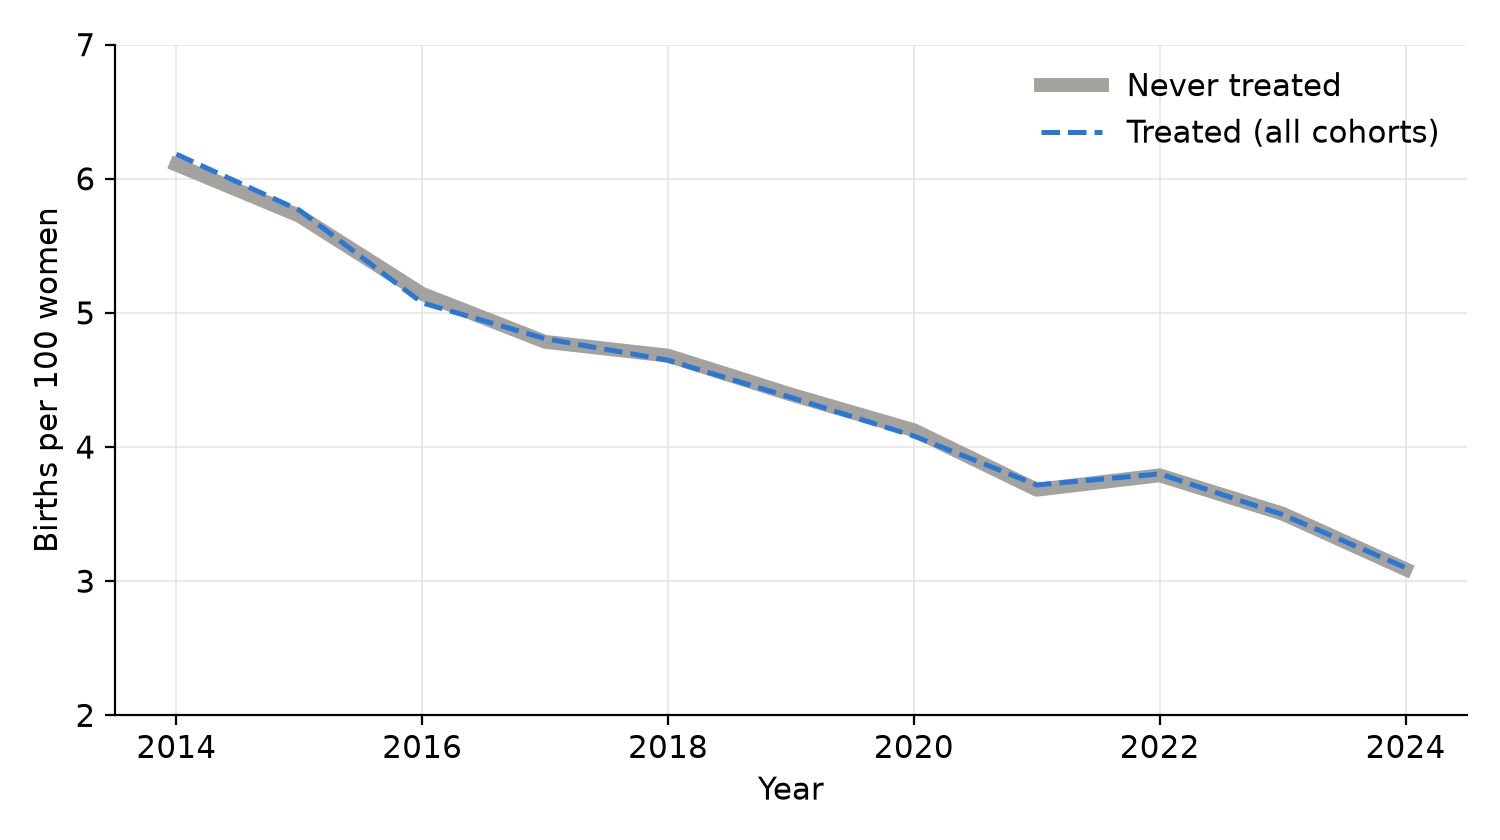
\includegraphics[width=\linewidth,height=0.60\textheight,keepaspectratio]{../RIS/20261104/graficos/en_fert_tasa.png}
\par\raggedright\fuente{Vulnerable women aged 18--49.}
\takeaway{Births per 100 women halve between 2014 and 2024, and treated and control fall together.}
\end{frame}

\begin{frame}{Fertility: no significant effect on births}
\begin{columns}[c]
\begin{column}{0.58\textwidth}
\centering
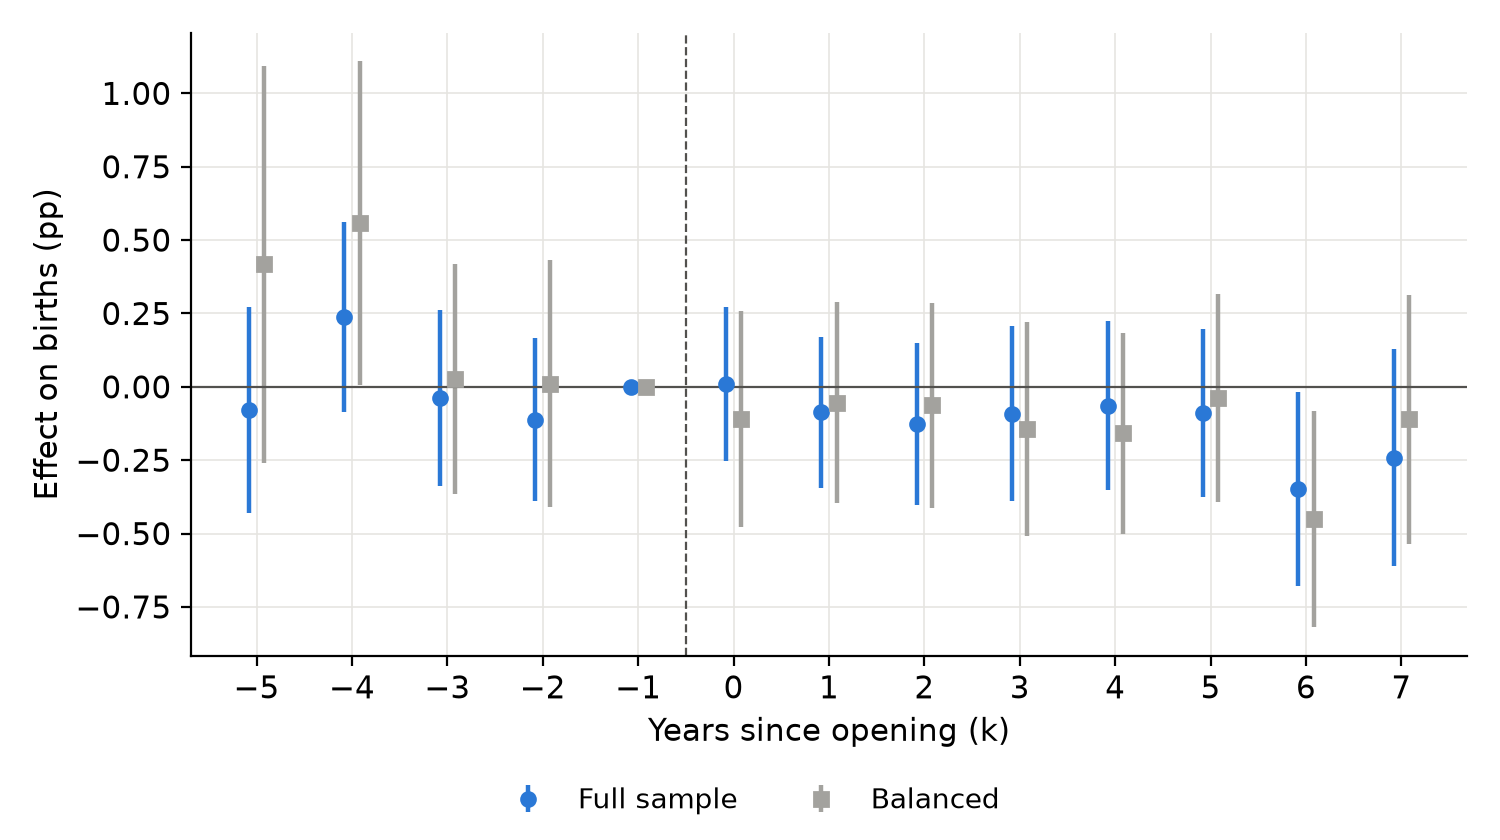
\includegraphics[width=\linewidth,height=0.62\textheight,keepaspectratio]{../RIS/20261104/graficos/en_fert.png}
\end{column}
\begin{column}{0.40\textwidth}
\begin{itemize}
  \footnotesize
  \item \textbf{Measure}: share of vulnerable women, 18--35 in 2014, who had a child that year
  \item \textbf{Start}: $\approx$6 births per 100 women a year, average 2014--2024
  \item \textbf{Pre-trends}: none ($p=0.25$, balanced $p=0.27$)
  \item \textbf{Estimate}, first 8 years: \textbf{$-$0.13pp} full, \textbf{$-$0.14pp} balanced, not significant
  \item Rules out falls above $\approx$6\% and rises above $\approx$2\%
  \item \textbf{Last meeting}: also no effect, with women 18--49
\end{itemize}
\end{column}
\end{columns}
\takeaway{We see no significant effect on births, and can rule out falls above about 6\%.}
\par\fuente{Sun--Abraham, weighted, 95\% CI clustered by UV, ref.\ $k=-1$.}
\end{frame}

\begin{frame}{Fertility, woman fixed effects}
\begin{columns}[c]
\begin{column}{0.58\textwidth}
\centering
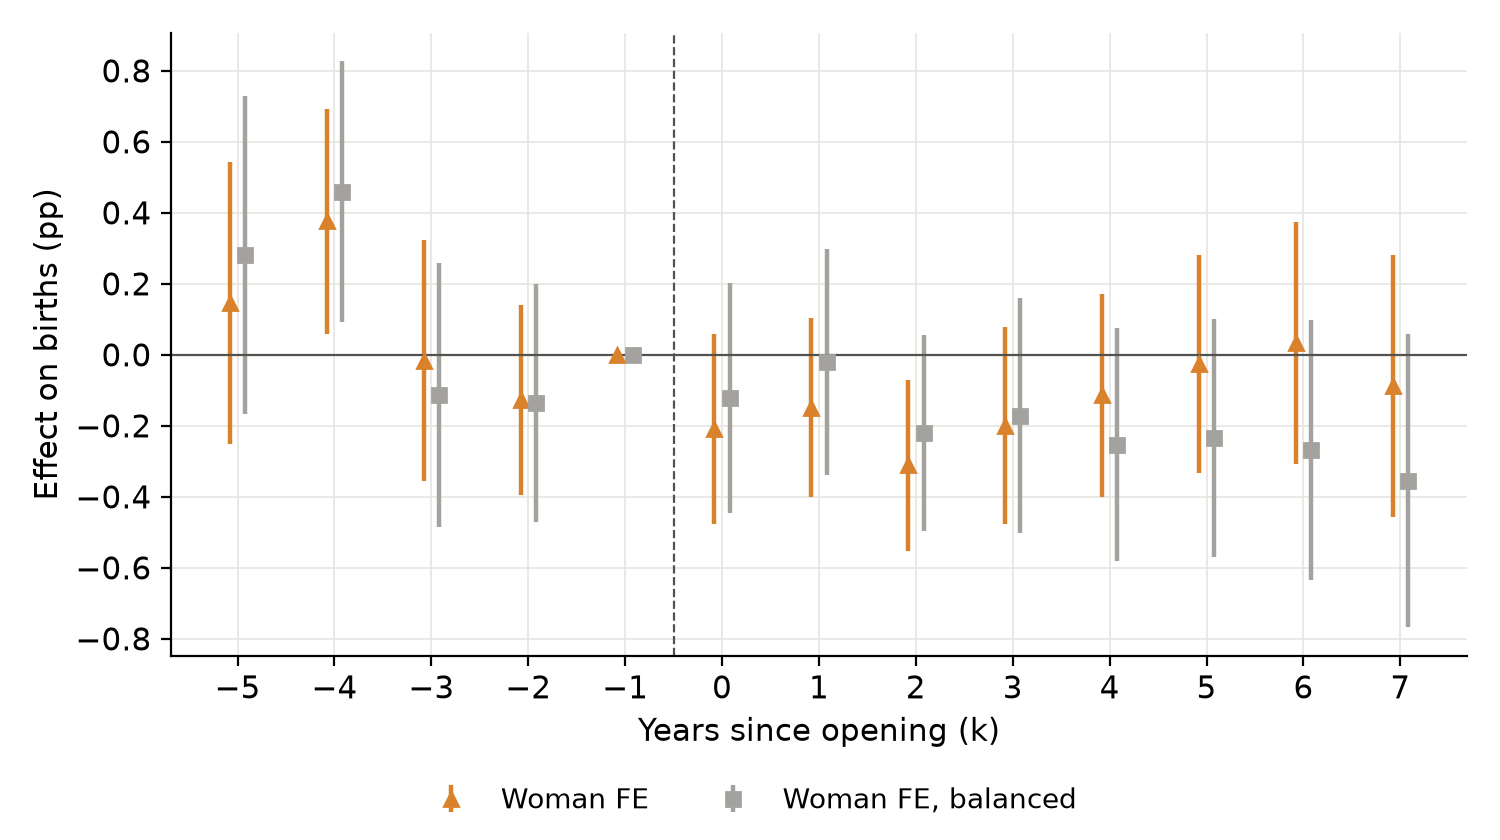
\includegraphics[width=\linewidth,height=0.62\textheight,keepaspectratio]{../RIS/20261104/graficos/en_fert_ef.png}
\end{column}
\begin{column}{0.40\textwidth}
\begin{itemize}
  \footnotesize
  \item \textbf{Woman fixed effects}: each woman compared with herself, in the first UV where she appears
  \item \textbf{Start}: $\approx$6 births per 100 women a year
  \item \textbf{Pre-trends}: yes ($p=0.01$, balanced $p<0.01$)
  \item \textbf{Estimate}, first 8 years: \textbf{$-$0.13pp}, \textbf{$-$0.21pp} balanced, not significant
\end{itemize}
\end{column}
\end{columns}
\takeaway{With woman fixed effects we see no significant effect either, and both versions have pre-trends.}
\par\fuente{Sun--Abraham, 95\% CI, ref.\ $k=-1$.}
\end{frame}

\begin{frame}{Fertility: cumulative births}
\begin{columns}[c]
\begin{column}{0.58\textwidth}
\centering
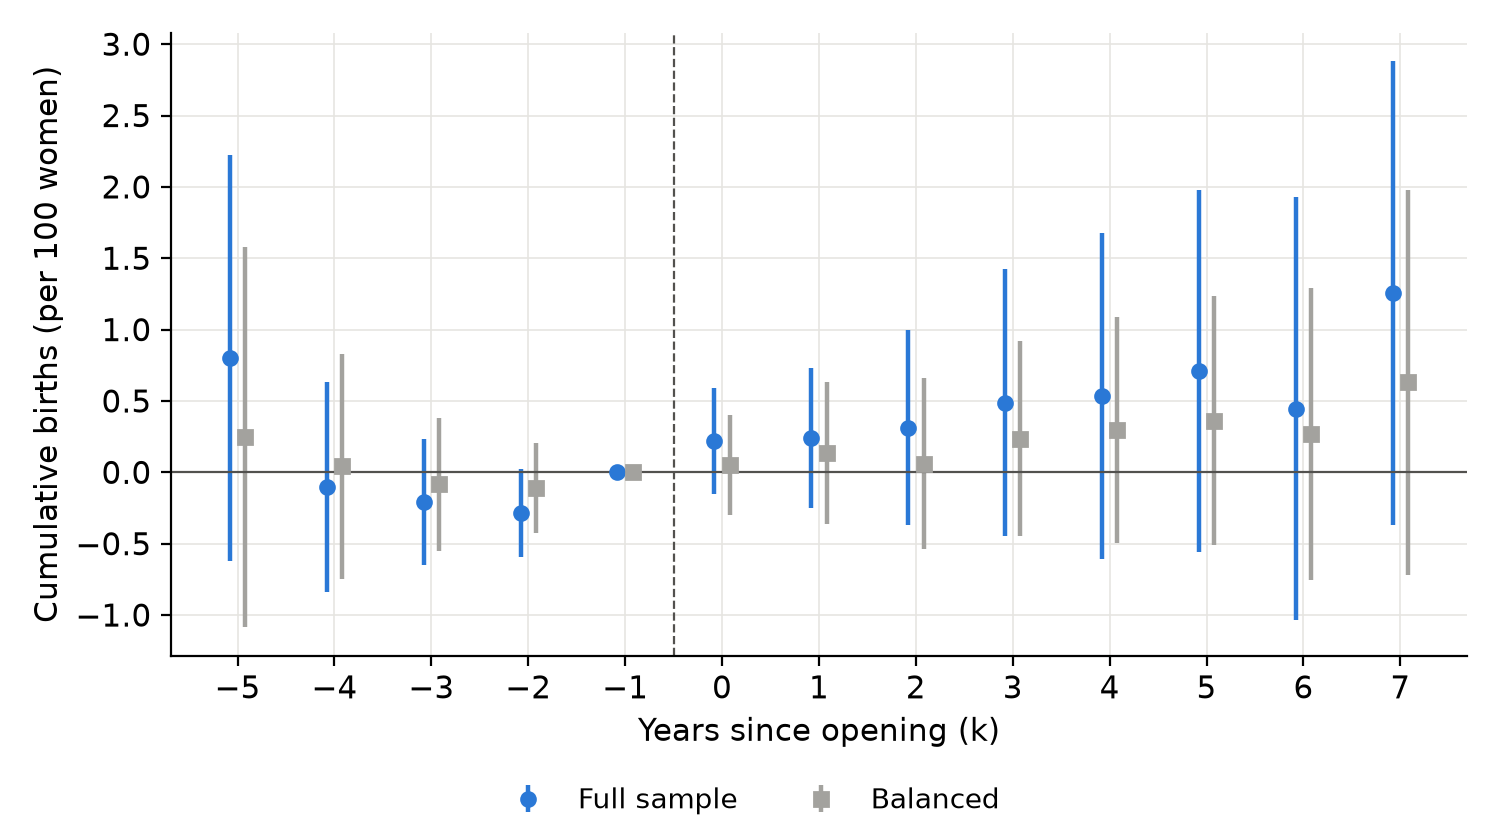
\includegraphics[width=\linewidth,height=0.62\textheight,keepaspectratio]{../RIS/20261104/graficos/en_nac.png}
\end{column}
\begin{column}{0.40\textwidth}
\begin{itemize}
  \footnotesize
  \item \textbf{Measure}: running count of each woman's births since she first appears in the data
  \item \textbf{Why}: the annual rate shows when women have children; this shows how many
  \item \textbf{Start}: $\approx$0.38 births per woman
  \item \textbf{Pre-trends}: none ($p=0.12$, balanced $p=0.94$)
  \item \textbf{Estimate}, first 8 years: \textbf{+0.5} full, \textbf{+0.3} balanced, per 100 women, not significant
  \item Woman FE: +0.3, with clear pre-trends; parallel trends here require equal birth \emph{rates} (appendix)
\end{itemize}
\end{column}
\end{columns}
\takeaway{The number of births does not change significantly: about half a birth more per 100 women.}
\par\fuente{Sun--Abraham, weighted, 95\% CI clustered by UV, ref.\ $k=-1$.}
\end{frame}

\begin{frame}{Fertility: total children}
\begin{columns}[c]
\begin{column}{0.58\textwidth}
\centering
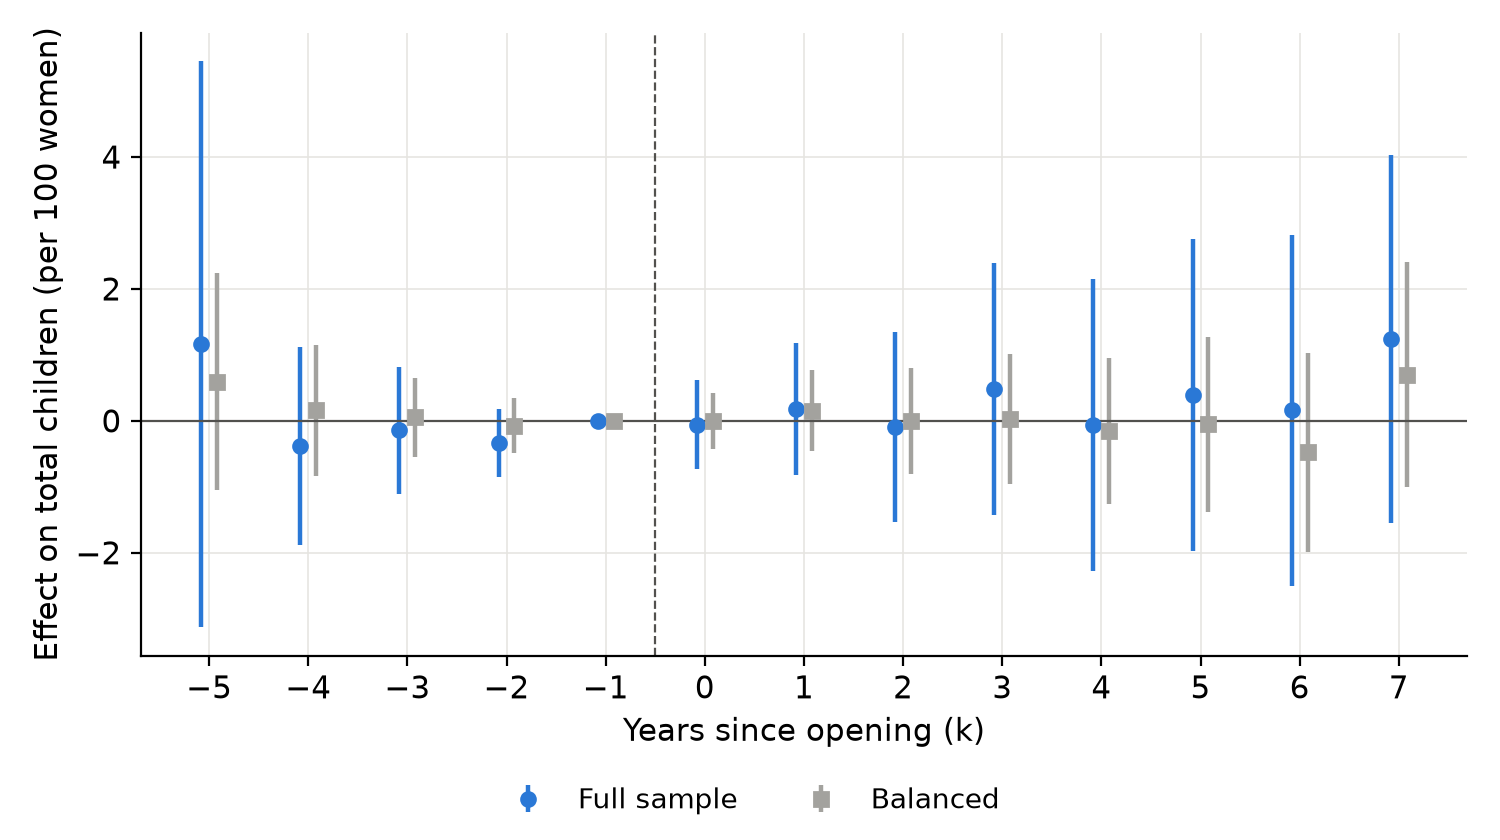
\includegraphics[width=\linewidth,height=0.62\textheight,keepaspectratio]{../RIS/20261104/graficos/en_hijos_total.png}
\end{column}
\begin{column}{0.40\textwidth}
\begin{itemize}
  \footnotesize
  \item \textbf{Measure}: children born before 2014 plus births since she first appears in the data
  \item \textbf{Why}: also counts the children she already had
  \item \textbf{Start}: $\approx$1.25 children per woman
  \item \textbf{Pre-trends}: none visible, no year stands out
  \item \textbf{Estimate}, first 8 years: \textbf{+0.3} full, \textbf{+0.03} balanced, per 100 women; no year is significant
\end{itemize}
\end{column}
\end{columns}
\takeaway{Counting the children women already had, we also see no significant change.}
\par\fuente{Sun--Abraham, weighted, 95\% CI clustered by UV, ref.\ $k=-1$.}
\end{frame}

\begin{frame}{Main conclusions so far}
\begin{itemize}
  \small
  \item \textbf{Enrollment}: rises right when the first preschool opens, from 34\% to 37\%
  \item \textbf{Employment}: more mothers enter formal work, gradually, from about 55\% to 56\%. All versions point the same way, at about half the size with woman fixed effects
  \item \textbf{Earnings including zeros}: mothers' average earnings in the UV rise about 3.6\%. Woman fixed effects suggest a smaller rise, around 1\%
  \item \textbf{Earnings of mothers with earnings}: the UV estimates suggest a rise, but it is not clear when following the same women
  \item \textbf{Fertility}: estimates are small and not significant, suggesting no large change in births
\end{itemize}
\takeaway{Openings bring children into preschool right away and mothers into formal work gradually, with no clear change in births.}
\end{frame}

% =============================================================================
% PENDING
% =============================================================================
\begin{frame}{What is pending}
\vspace{-4pt}
\begin{center}
\scriptsize
\renewcommand{\arraystretch}{0.95}
\setlength{\tabcolsep}{4pt}
\begin{tabular}{@{}l>{\raggedright\arraybackslash}p{6.6cm}>{\raggedright\arraybackslash}p{4.4cm}@{}}
\toprule
\textbf{Meeting} & \textbf{Topic} & \textbf{Status} \\
\midrule
Oct 29 & Mothers enter at first appearance; balanced women & \textcolor{statuslisto}{\textbf{Done}} \\
Oct 29 & Fertility outcome: cumulative births, total children & \textcolor{statuslisto}{\textbf{Done}} \\
Oct 29 & Fertility outcome: number of births in the UV & \textcolor{statusred}{\textbf{Pending}} \\
Oct 15 & Moves in 2022 & \textcolor{statuspink}{\textbf{Open}}: UV fixed from 2022 running \\
Oct 22 & All women, not only mothers (labor) & \textcolor{statuspink}{\textbf{Running}} \\
Oct 22 & Include UVs with preschools in 2014 (Callaway--Sant'Anna) & \textcolor{statuspink}{\textbf{Running}} \\
Oct 15 & Effects by child's age at opening & \textcolor{statuspink}{\textbf{Running}} \\
Oct 15 & Spillovers to neighboring UVs (fertility) & \textcolor{statuspink}{\textbf{Running}} \\
Oct 22 & Earlier years for pre-trends & \textcolor{statuspink}{\textbf{Availability checked}} \\
--- & Sensitivity to pre-trends (HonestDiD) & \textcolor{statusred}{\textbf{Next}} \\
Oct 15 & First stage for the other 40\% & \textcolor{statusred}{\textbf{Pending}} \\
Oct 15 & Who fills the new preschool; extended hours & \textcolor{statusred}{\textbf{Pending}} \\
Oct 8 & Treatment by initial stock of preschools & \textcolor{statusred}{\textbf{Not started}} \\
Oct 8 & Sample by predicted probability of pregnancy & \textcolor{statusred}{\textbf{Not started}} \\
\bottomrule
\end{tabular}
\end{center}
\takeaway{Sample changes are done; robustness is running; mechanisms and the 2022 jump come next.}
\end{frame}

% =============================================================================
% APPENDIX
% =============================================================================
\appendix
% Appendix: page number without total, so the main deck shows only the main count
\setbeamertemplate{footline}{
  \hfill
  \raisebox{6pt}{\textcolor{graytext}{\scriptsize Appendix \insertframenumber}}
  \hspace{10pt}
  \vspace{6pt}
}
\begin{frame}[plain]
\vspace{60pt}
\begin{center}
{\LARGE\bfseries\color{navy} Appendix}
\end{center}
\end{frame}

\begin{frame}{Appendix A1. Fertility by children before 2014 (exploratory)}
\centering
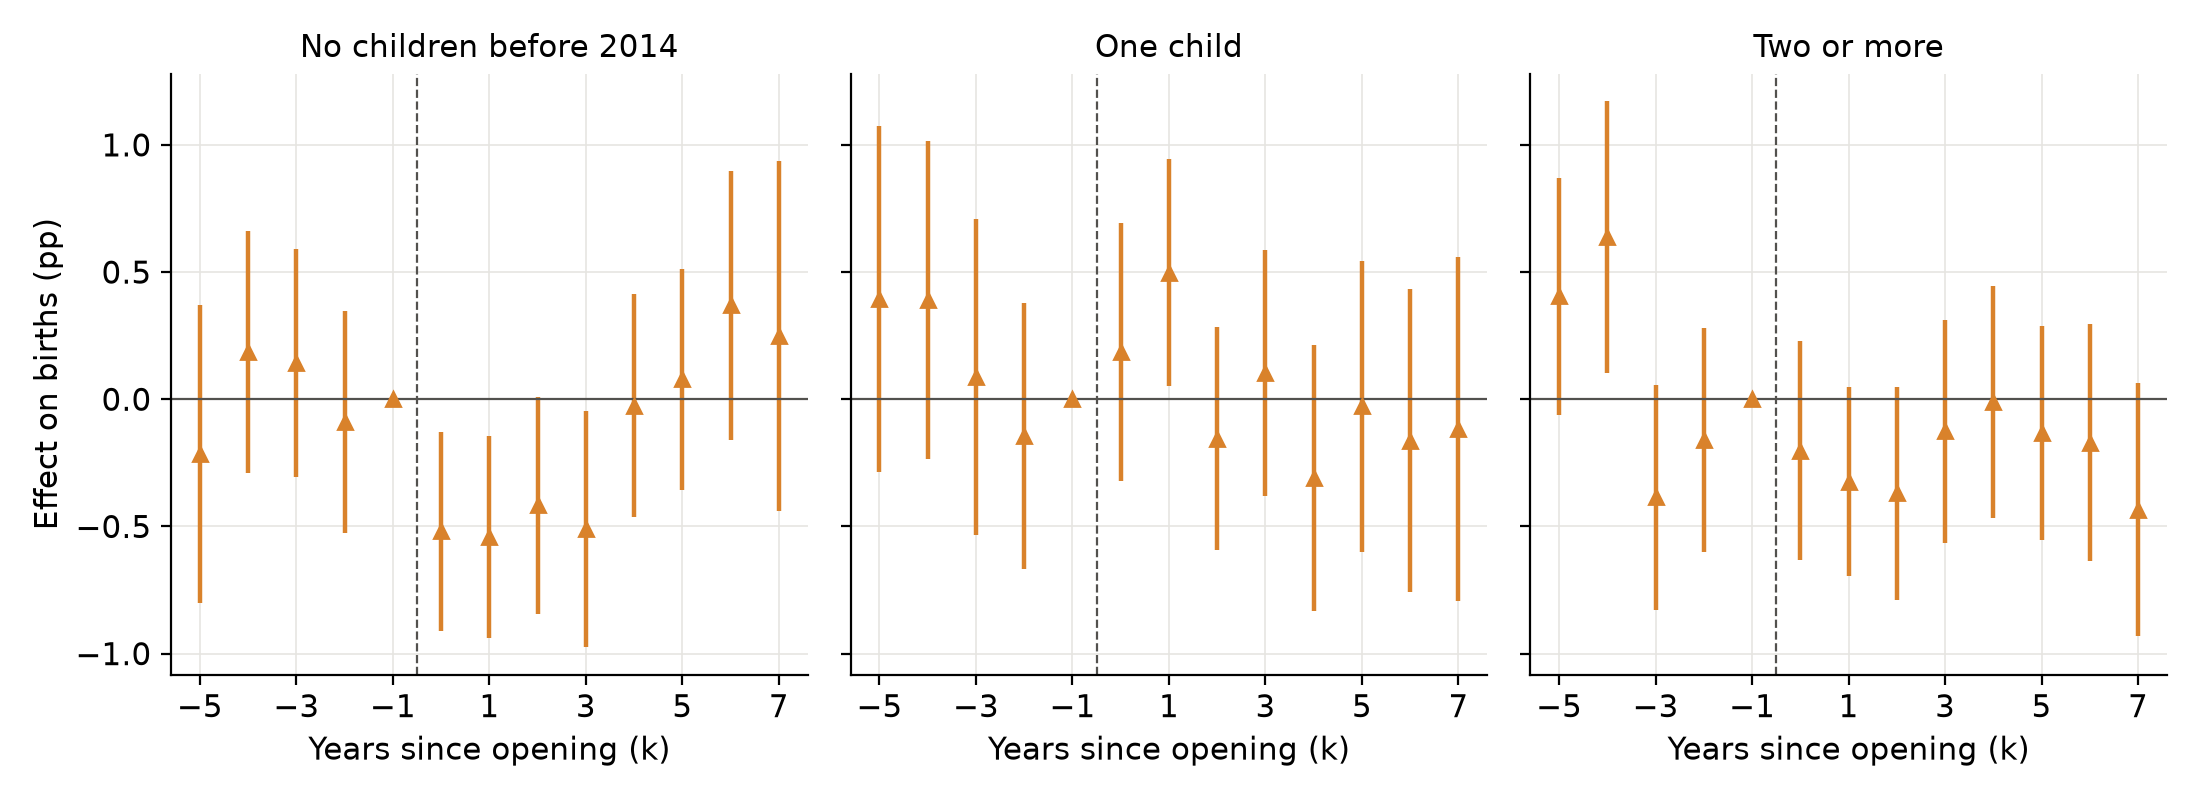
\includegraphics[width=\linewidth,height=0.48\textheight,keepaspectratio]{../RIS/20261104/graficos/en_fert_hijos.png}
\raggedright
\begin{itemize}
  \footnotesize
  \item Woman FE. Each panel is a separate regression: treated vs.\ control with the same children before 2014; group is fixed
  \item No children before 2014: $\approx-$0.5pp the first four years (base 6.1), then back to zero
\end{itemize}
\takeaway{A signal among women without previous children, but it is not repeated at the UV level and starts in the opening year.}
\end{frame}

\begin{frame}{Appendix A2. Why a cumulative outcome has pre-trends more easily}
\noindent{\footnotesize Example with \textbf{no effect}: control 6.0 births per 100 women every year, treated 5.8 every year.}
\vspace{4pt}
\begin{center}
\footnotesize
\begin{tabular}{@{}lccccccc@{}}
\toprule
$k$ & $-$4 & $-$3 & $-$2 & $-$1 & 0 & 1 & 2 \\
\midrule
Gap in the rate & $-$0.2 & $-$0.2 & $-$0.2 & $-$0.2 & $-$0.2 & $-$0.2 & $-$0.2 \\
\textbf{Coefficient, rate} & 0 & 0 & 0 & 0 & 0 & 0 & 0 \\
\midrule
Gap in cumulative births & $-$0.2 & $-$0.4 & $-$0.6 & $-$0.8 & $-$1.0 & $-$1.2 & $-$1.4 \\
\textbf{Coefficient, cumulative} & +0.6 & +0.4 & +0.2 & 0 & $-$0.2 & $-$0.4 & $-$0.6 \\
\bottomrule
\end{tabular}
\end{center}
\begin{itemize}
  \footnotesize
  \item For the rate, the gap only needs to be stable
  \item For the cumulative outcome, the gap is constant only if both groups have exactly the same rate
  \item If treated had 6.2 instead, the line would rise after the opening with no effect at all
\end{itemize}
\takeaway{A small stable gap in birth rates looks like a pre-trend, or an effect, in cumulative births.}
\end{frame}

\begin{frame}{Appendix A3. Balance in 2014}
\begin{center}
\footnotesize
\begin{tabular}{@{}lccc@{}}
\toprule
 & Never treated & Treated & Std.\ difference \\
\midrule
Formal employment & 55.5\% & 55.8\% & 0.03 \\
Monthly earnings, mothers with earnings (2014 pesos) & CLP 296k & CLP 298k & 0.02 \\
Months with earnings & 8.2 & 8.1 & $-$0.03 \\
Age & 27.9 & 28.1 & 0.13 \\
Children under 5 & 0.68 & 0.69 & 0.16 \\
Child density in the UV & 0.061 & 0.064 & 0.20 \\
\textbf{Mothers per UV} & 286 & 520 & \textbf{0.50} \\
\textbf{UV population} & 3,198 & 5,332 & \textbf{0.44} \\
\bottomrule
\end{tabular}
\end{center}
\par\fuente{Labor sample, weighted by UV population. 299 treated and 3,811 never treated UVs with data in 2014; 2014 UV is the 2016 UV.}
\takeaway{Mothers look alike in 2014; what differs is UV size.}
\end{frame}

\begin{frame}{Appendix A4. Woman fixed effects: specification}
\[
E_{it} \;=\; \mu_i \;+\; \lambda_t \;+\; \sum_{k \neq -1} \beta_k \, \mathbf{1}\{\, t - G_{u_0(i)} = k \,\} \;+\; \varepsilon_{it}
\]
\vspace{-4pt}
\begin{center}
\colorbox{bgpanel}{\parbox{0.92\linewidth}{\scriptsize\ttfamily
eventstudyinteract empleo\_formal d1-d4 d6-d15, cohort(g1\_f) control\_cohort(nunca\_f) \\
\hspace*{2em}absorb(rut\_inn anio) vce(cluster uv\_fija)}}
\end{center}
\vspace{-4pt}
\begin{columns}[T]
\begin{column}{0.52\textwidth}
\begin{itemize}
  \footnotesize
  \item $E_{it}$: formal employment of mother $i$ in year $t$
  \item $\mu_i$: \textbf{woman} fixed effect; $\lambda_t$: year fixed effect
  \item $u_0(i)$: \textbf{fixed UV} = first valid UV where the mother appears, before the opening
  \item $G_{u_0(i)}$: year her fixed UV opens its first preschool $\to$ kept even if she moves
\end{itemize}
\end{column}
\begin{column}{0.46\textwidth}
\begin{itemize}
  \footnotesize
  \item \textbf{Sun--Abraham}: cohorts by $G_{u_0(i)}$ (\texttt{g1\_f}); controls = fixed UV never opens one (\texttt{nunca\_f})
  \item $k \leq -5$ binned; ref.\ $k=-1$; SE clustered by fixed UV
  \item Sample: vulnerable mothers whose fixed UV had no preschool in 2014, first observed before the opening
\end{itemize}
\end{column}
\end{columns}
\takeaway{Each mother is compared with herself, treated by the first UV where she appears.}
\par\fuente{$\approx$5.6M mother-years.}
\end{frame}

\begin{frame}{Appendix A5. More pre-trend years: how far back can we go?}
\begin{columns}[T]
\begin{column}{0.54\textwidth}
\begin{center}
\footnotesize
\begin{tabular}{@{}llr@{}}
\toprule
Source & Outcome & From \\
\midrule
FPS (women, household) & sample, UV & 2007 \\
Preschool enrollment & first stage & 2011 \\
Earnings (SII, historical) & labor & 2002 \\
Contributions (AFP) & labor & 2015 \\
Civil Registry births & fertility & no limit \\
\bottomrule
\end{tabular}
\end{center}
\vspace{2pt}
{\footnotesize \textbf{Proposal}: start in \textbf{2011} $\to$ 3 more pre-years for every cohort (the 2015 cohort goes from 1 to 4). Labor 2011--2013: earnings only.}
\end{column}
\begin{column}{0.42\textwidth}
\colorbox{bgpanel}{\parbox{0.95\linewidth}{\raggedright\footnotesize
\textbf{The catch: UVs before 2016}
\begin{itemize}
  \footnotesize
  \item FPS has \textbf{no reliable UV} code
  \item Our crosswalk only reaches back to 2016
  \item Pre-2016 years must be anchored to the woman's \textbf{2016 UV} $\to$ women who left before 2016 are lost, and earlier moves are invisible
\end{itemize}}}
\end{column}
\end{columns}
\takeaway{Data exist back to 2011 for all outcomes, but UVs before 2016 have to be proxied by the 2016 UV.}
\end{frame}

\begin{frame}{Appendix A6. Full identification assumptions and placebo check}
\begin{itemize}
  \item \textbf{Parallel trends}: assessed via pre-opening event-study coefficients; should be statistically indistinguishable from zero
  \item \textbf{No anticipation}: mothers do not adjust decisions before the effective opening --- depends on how much advance notice openings receive (to analyze)
  \item \textbf{Exogeneity of timing}: opening timing should not correlate with unobserved UV characteristics. \textbf{Main threat}: JUNJI/Integra may prioritize UVs with higher care demand or specific socioeconomic profiles
\end{itemize}

\vspace{10pt}
\begin{block}{Placebo check}
\small An analogous event study will be estimated using the \textbf{pre-treatment birth rate} of the UV as the outcome. Non-significant pre-treatment coefficients would strengthen the parallel-trends assumption of the main model.
\end{block}
\end{frame}

\begin{frame}{Appendix A7. Data limitation: UV assignment in 2014--2015}
\begin{itemize}
  \item FPS (2014--2015) has no reliable UV field $\to$ those two years are anchored to the woman's \textbf{2016 UV} as a proxy
  \item \textbf{Consequence}: women who left the panel before 2016 are dropped from 2014--2015 --- precisely the earliest pre-trend years
  \item RIS has not delivered a better historical crosswalk despite repeated requests; only unstandardized UV name strings are available
  \item \textbf{Idea, not yet tested}: fuzzy matching on UV name strings
\end{itemize}
\end{frame}

\begin{frame}{Appendix A8. Two ways to measure earnings}
\noindent{\footnotesize Example: a UV with 4 mothers. After the opening, \textbf{C starts working}, at a somewhat lower wage (CLP million per year).}
\vspace{4pt}
\begin{center}
\footnotesize
\renewcommand{\arraystretch}{1.2}
\begin{tabular}{@{}lccccc|c|c@{}}
\toprule
 & A & B & C & D & & \textbf{Earnings incl.\ zeros} & \textbf{ln earnings} \\
 & & & & & & \textcolor{graytext}{(all mothers)} & \textcolor{graytext}{(only mothers who work)} \\
\midrule
Before & 4 & 4 & 0 & 0 & & (4+4+0+0)/4 = \textbf{2.0} & mean of A, B = 4 \\
After & 4 & 4 & \textbf{3} & 0 & & (4+4+3+0)/4 = \textbf{2.75} $\uparrow$ & mean of A, B, C $\approx$ 3.6 $\downarrow$ \\
\bottomrule
\end{tabular}
\end{center}
\vspace{4pt}
\begin{columns}[T]
\begin{column}{0.48\textwidth}
\begin{itemize}
  \footnotesize
  \item \textbf{Earnings including zeros}: how much income mothers have \emph{overall} $\to$ rises if more mothers work \emph{or} if they earn more
  \item Expressed relative to the year's mean (100): +2 points $\approx$ +2\% for the average mother
\end{itemize}
\end{column}
\begin{column}{0.48\textwidth}
\begin{itemize}
  \footnotesize
  \item \textbf{ln earnings}: how much \emph{working} mothers earn $\to$ can fall when new workers enter with lower wages, even if no one's wage falls
\end{itemize}
\end{column}
\end{columns}
\takeaway{Earnings including zeros capture new workers; ln earnings only captures wages.}
\end{frame}

\begin{frame}{Appendix A9. Research question}
\begin{block}{Question}
\small What are the effects of the public expansion of early childhood education in Chile on mothers' labor market participation and fertility?
\end{block}

\vspace{4pt}
\begin{columns}[T]
\begin{column}{0.49\textwidth}
{\small\textcolor{steel}{\textbf{What we know}}}
\begin{itemize}
  \footnotesize
  \item \textbf{Mixed evidence}: positive effects on maternal employment in Quebec and Argentina, close to zero in Norway
  \item Recent Latin American evidence comes from \textbf{lotteries and experiments} (Rio de Janeiro, Nicaragua)
  \item Less is known about a \textbf{national, decade-long public expansion} observed in administrative data
\end{itemize}
\end{column}
\begin{column}{0.49\textwidth}
{\small\textcolor{steel}{\textbf{Our contribution}}}
\begin{itemize}
  \footnotesize
  \item \textbf{First study to use neighborhood-unit (UV) variation}: preschools geolocated to the UV and linked to individual administrative records
  \item \textbf{Fertility} as a second margin, alongside labor supply
\end{itemize}

\vspace{4pt}
\colorbox{bgpanel}{\parbox{0.95\linewidth}{\raggedright\footnotesize \textbf{\textcolor{steel}{What is a UV?}} \emph{Unidad Vecinal}: the official sub-municipal territorial unit --- $\sim$6{,}900 UVs vs.\ 346 municipalities.}}
\end{column}
\end{columns}

\takeaway{Finer geography: a sharper measure of exposure and more variation to identify the effect.}
\par\vspace{10pt}
{\tiny\textcolor{graytext}{Quebec: Baker et al.\ (2008); Argentina: Berlinski \& Galiani (2007); Norway: Havnes \& Mogstad (2011); Rio: Attanasio et al.\ (2025); Nicaragua: Hojman \& L\'opez B\'oo (2022).}\par}
\end{frame}

\begin{frame}{Appendix A10. Public provision expanded sharply between 2015 and 2024}
\begin{itemize}
  \footnotesize
  \item Mixed provision: \textbf{public} (JUNJI, Integra, municipal/SLEP) vs. \textbf{private} (subsidized/paid)
  \item \textbf{700+ new public preschools} opened between 2015 and 2024
  \item Net attendance rate (ages 0--5) rose from \textbf{50\% to 55\%} over the period, despite pandemic-era setbacks
\end{itemize}

\vspace{6pt}
\begin{center}
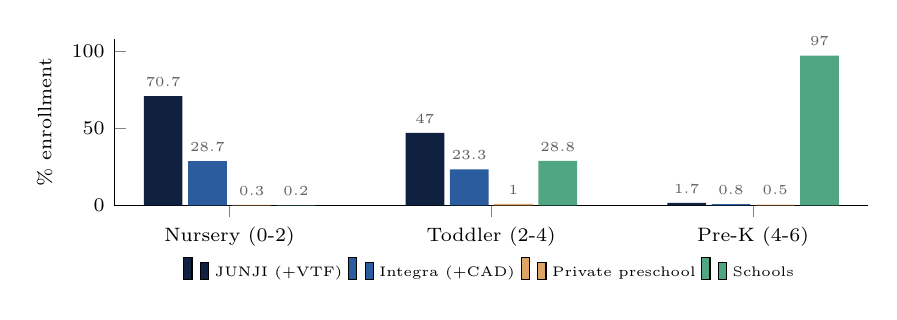
\begin{tikzpicture}
\begin{axis}[
  ybar,
  bar width=14pt,
  width=0.92\textwidth,
  height=3.7cm,
  symbolic x coords={Sala cuna,Nivel medio,Nivel transicion},
  xtick=data,
  xticklabels={Nursery (0-2),Toddler (2-4),Pre-K (4-6)},
  ymin=0, ymax=108,
  ylabel={\% enrollment},
  ylabel style={font=\scriptsize},
  tick label style={font=\scriptsize},
  axis lines*=left,
  enlarge x limits=0.22,
  nodes near coords,
  nodes near coords style={font=\tiny,text=graytext},
  legend style={at={(0.5,-0.27)},anchor=north,legend columns=4,font=\tiny,draw=none},
  grid style={gray!20},
]
\addplot[fill=navy,draw=none] coordinates {(Sala cuna,70.7)(Nivel medio,47.0)(Nivel transicion,1.7)};
\addplot[fill=steel,draw=none] coordinates {(Sala cuna,28.7)(Nivel medio,23.3)(Nivel transicion,0.8)};
\addplot[fill=psuborange,draw=none] coordinates {(Sala cuna,0.3)(Nivel medio,1.0)(Nivel transicion,0.5)};
\addplot[fill=schoolgreen,draw=none] coordinates {(Sala cuna,0.2)(Nivel medio,28.8)(Nivel transicion,97.0)};
\legend{JUNJI (+VTF), Integra (+CAD), Private preschool, Schools}
\end{axis}
\end{tikzpicture}
\end{center}
\vspace{-12pt}
\fuente{Source: authors' elaboration based on Figura 5, Matr\'icula Oficial 2023, Centro de Estudios MINEDUC.}
\takeaway{Ages 0--4: JUNJI and Integra are the main providers --- our focus.}
\end{frame}

\begin{frame}{Appendix A11. Identification: staggered-adoption event study}
\begin{columns}[T]
\begin{column}{0.66\textwidth}
\begin{itemize}
  \small
  \item \textbf{Design}: staggered-adoption difference-in-differences with event study
  \item \textbf{Unit of treatment}: the UV, the year it opens its first public preschool
  \item \textbf{Unit of analysis}: \textbf{UV $\times$ year} panel, built from a woman $\times$ year panel linked to each woman's UV of residence
  \item \textbf{Fixed effects}: \textbf{UV + year} (baseline); woman FE on the woman $\times$ year panel as a \textbf{robustness check}
  \item \textbf{Estimand}: ATT of UV-level treatment (Baker et al., \emph{JEL} 2026) --- an \textbf{intent-to-treat effect of access}, not individual take-up
\end{itemize}
\end{column}
\begin{column}{0.32\textwidth}
\centering
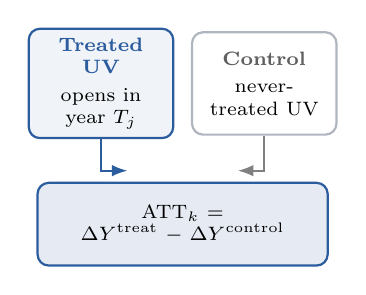
\begin{tikzpicture}[font=\scriptsize]
\node[draw=steel,thick,fill=bgpanel,rounded corners,text width=1.6cm,align=center,minimum height=1.3cm] (a) {\textbf{\textcolor{steel}{Treated UV}}\\[2pt]opens in year $T_j$};
\node[draw=neutralgray,thick,fill=white,rounded corners,text width=1.6cm,align=center,minimum height=1.3cm,right=6pt of a] (b) {\textbf{\textcolor{graytext}{Control}}\\[2pt]never-treated UV};
\coordinate (mid) at ($(a.south)!0.5!(b.south)$);
\node[draw=steel,thick,fill=steel!12,rounded corners,text width=3.45cm,align=center,minimum height=1.05cm,below=16pt of mid] (c) {ATT$_k$ = $\Delta Y^{\text{treat}} - \Delta Y^{\text{control}}$};
\draw[-{Latex[length=2mm]},steel,thick] (a.south) |- ($(c.north)+(-0.7,4pt)$);
\draw[-{Latex[length=2mm]},gray,thick] (b.south) |- ($(c.north)+(0.7,4pt)$);
\end{tikzpicture}
\end{column}
\end{columns}
\takeaway{We compare changes in UVs that get their first preschool vs.\ UVs that never do --- an intent-to-treat effect of access.}
\end{frame}

\begin{frame}{Appendix A12. A UV is treated when it opens its first preschool}
\begin{block}{Treatment definition}
\small A UV is \textbf{treated} the year it opens its first public preschool (JUNJI/Integra) --- goes from 0 to 1+ centers.
\end{block}

\vspace{8pt}
\begin{center}
\small
\begin{tabular}{@{}lp{6.4cm}rr@{}}
\toprule
\textbf{Group} & \textbf{Definition} & \textbf{N (UVs)} & \textbf{\%} \\
\midrule
Excluded        & Already had 1+ center in 2014 (out of design)      & 2{,}394 & 34.8\% \\
Never-treated   & 0 in 2014, stays at 0 through 2024                 & 4{,}174 & 60.6\% \\
Treated         & 0 in 2014, opens first center 2015--2024           & 319     & 4.6\%  \\
\midrule
\textbf{Total universe} & & \textbf{6{,}887} & 100\% \\
\end{tabular}
\end{center}
\fuente{Source: \texttt{base\_cobertura\_cp.dta}, corrected opening years (Oct 21). Design sample (\texttt{muestra\_t1==1}) = 4{,}493 UVs. Previous version: 447 treated, 2{,}265 excluded.}
\takeaway{We identify the effect of the first preschool (0 $\to$ 1): 319 treated vs.\ 4{,}174 never-treated.}
\end{frame}

\begin{frame}{Appendix A13. Treatment cohorts by year}
\begin{columns}[T]
\begin{column}{0.56\textwidth}
\centering
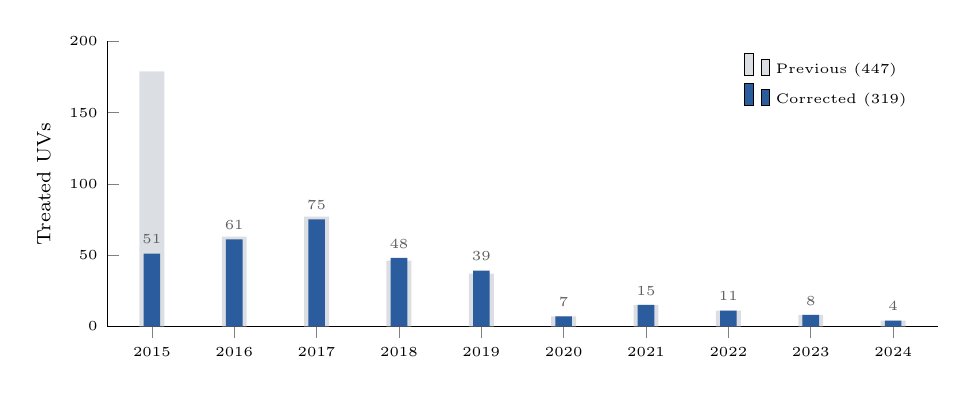
\begin{tikzpicture}
\begin{axis}[
  ybar,
  bar width=9pt,
  width=\linewidth,
  height=5.2cm,
  symbolic x coords={2015,2016,2017,2018,2019,2020,2021,2022,2023,2024},
  xtick=data,
  ymin=0, ymax=200,
  ylabel={Treated UVs},
  ylabel style={font=\scriptsize},
  tick label style={font=\tiny},
  axis lines*=left,
  enlarge x limits=0.06,
  legend style={font=\tiny,draw=none,at={(0.98,0.98)},anchor=north east},
  legend cell align=left,
]
\addplot[fill=neutralgray!45,draw=none,bar shift=0pt] coordinates {(2015,179)(2016,63)(2017,77)(2018,46)(2019,37)(2020,7)(2021,15)(2022,11)(2023,8)(2024,4)};
\addplot[fill=steel,draw=none,bar shift=0pt,bar width=6pt,nodes near coords,nodes near coords style={font=\tiny,text=graytext}] coordinates {(2015,51)(2016,61)(2017,75)(2018,48)(2019,39)(2020,7)(2021,15)(2022,11)(2023,8)(2024,4)};
\legend{Previous (447),Corrected (319)}
\end{axis}
\end{tikzpicture}
\end{column}
\begin{column}{0.42\textwidth}
\begin{itemize}
  \footnotesize
  \item \textbf{2015 cohort corrected}: 179 $\to$ \textbf{51 UVs} --- in 127 UVs the ``opening'' was a center already operating in 2014 (next slide)
  \item Other cohorts barely change; \textbf{2017 is now the largest} (75 UVs)
  \item \textbf{59\% open in 2015--2017}; only 45 UVs open after 2019
  \item The 2015 cohort still has \textbf{only one pre-period} (2014)
\end{itemize}
\end{column}
\end{columns}
\fuente{Source: \texttt{base\_cobertura\_cp.dta}, corrected opening years (Oct 21). 319 treated UVs (0 centers in 2014).}
\takeaway{Openings are spread over 2015--19, no longer concentrated in 2015.}
\end{frame}

\begin{frame}{Appendix A14. Most 2015 ``openings'' were centers already operating}
\begin{columns}[T]
\begin{column}{0.52\textwidth}
\footnotesize
\begin{itemize}[itemsep=3pt]
  \item \textbf{Problem}: JUNJI opening dates come from records that start in March 2015 $\to$ centers with no earlier record were dated \textbf{01-03-2015} (84\% of 2015 openings)
  \item \textbf{Evidence}: older transparency requests give \textbf{center $\times$ year panels} (JUNJI 1996--2023, Integra 2001--2024); JUNJI centers are flat at $\sim$3{,}150 a year in 2011--2016
  \item \textbf{Fix}: opening year = first year the center appears in the panels
\end{itemize}
\end{column}
\begin{column}{0.44\textwidth}
\centering
\scriptsize
JUNJI centers ``opening'' in 2015\\[3pt]
\begin{tabular}{@{}lrr@{}}
\toprule
Recorded date & Centers & Already there \\
\midrule
01-03-2015 & 444 & \textbf{427 (96\%)} \\
Other 2015 date & 108 & 15 (14\%) \\
\bottomrule
\end{tabular}

\vspace{10pt}
\begin{tabular}{@{}lrr@{}}
\toprule
UVs & Before & After \\
\midrule
Treated & 447 & \textbf{319} \\
\quad 2015 cohort & 179 & \textbf{51} \\
Excluded (center in 2014) & 2{,}265 & 2{,}394 \\
Never-treated & 4{,}175 & 4{,}174 \\
\bottomrule
\end{tabular}
\end{column}
\end{columns}

\vspace{4pt}
\begin{block}{Done: everything re-estimated with the corrected treatment}
\scriptsize
All results in the main slides use the corrected treatment (319 treated UVs). Previous results are in the appendix.
\end{block}
\takeaway{The 2015 cohort was mostly a data artifact: 127 of its 179 UVs already had a center in 2014.}
\end{frame}

\begin{frame}{Appendix A15. Empirical specification and estimator}
\[
Y_{ut} = \lambda_u + \lambda_t + \gamma\,\overline{\text{Age}}_{ut} + \sum_{k \neq -1} \beta_k \, \mathbf{1}\{t - G_u = k\} + \varepsilon_{ut}
\]

\vspace{2pt}
\begin{itemize}
  \footnotesize
  \item $Y_{ut}$: average outcome of women in UV $u$, year $t$ (built from the woman $\times$ year panel). $\lambda_u,\lambda_t$: UV and year fixed effects; SE clustered by UV.
  \item $\overline{\text{Age}}_{ut}$: average age of mothers in the UV-year (labor market specification).
  \item $\beta_k$: effect $k$ years from opening, relative to $k=-1$ (omitted); $k \le -5$ binned.
\end{itemize}

\vspace{4pt}
\begin{block}{Estimation strategy}
\footnotesize \textbf{Baseline TWFE} as reference --- but with staggered treatment, TWFE can use already-treated units as controls (Goodman-Bacon problem). Robust estimator: \textbf{Sun--Abraham} (\texttt{eventstudyinteract}), never-treated UVs as control group. Framework: Baker, Callaway, Cunningham, Goodman-Bacon \& Sant'Anna (\emph{JEL}, 2026).
\end{block}

\vspace{4pt}
\footnotesize \textbf{Main threat}: non-random placement of openings (JUNJI/Integra prioritizing UVs by care demand or socioeconomic profile). \textbf{UV FE} absorb permanent differences across UVs; \textbf{pre-period coefficients} ($k<-1$) test whether trends were already diverging.

\takeaway{Main estimator: Sun--Abraham with never-treated UVs as controls; TWFE as reference.}
\end{frame}

\begin{frame}{Appendix A16. Data: what we have and how each sample is built}
\small
\begin{center}
\renewcommand{\arraystretch}{1.35}
\begin{tabular}{@{}>{\raggedright\arraybackslash}p{2.8cm}>{\raggedright\arraybackslash}p{5.0cm}>{\raggedright\arraybackslash}p{4.6cm}@{}}
\toprule
\textbf{Sample} & \textbf{Source data} & \textbf{Key variables} \\
\midrule
Coverage (UV $\times$ year) & JUNJI/Integra transparency requests + UV shapefile (MDSF) & Number of centers, treatment status, opening cohort \\
Women panel (base) & RSH (2016--2024) + FPS (2014--2015) & UV of residence, UV population, child density \\
Labor market & + Rentas (SII/AFC) + Cotizaciones (AFP) & Annual income, months worked, employment \\
Fertility & + Civil Registry birth records (via RIS) & Birth in the year, children under 5 \\
First stage (enrollment) & + Matr\'icula parvularia (child-level) & Enrollment, enrollment rate \\
\bottomrule
\end{tabular}
\end{center}
\takeaway{All administrative registries, linked at the individual level --- no survey self-reports.}
\end{frame}

\begin{frame}{Appendix A17. Every preschool is matched to its 2024 neighborhood unit}
\begin{columns}[T]
\begin{column}{0.38\textwidth}
\begin{itemize}
  \footnotesize
  \item Each JUNJI/Integra preschool is \textbf{geolocated} and matched to the UV where it sits (spatial join)
  \item UV boundaries \textbf{changed a lot} over time $\to$ we traced them and mapped everything to \textbf{2024 boundaries}
  \item Preschools and women's UV of residence share \textbf{one common geography} across all years
\end{itemize}
\end{column}
\begin{column}{0.60\textwidth}
\centering
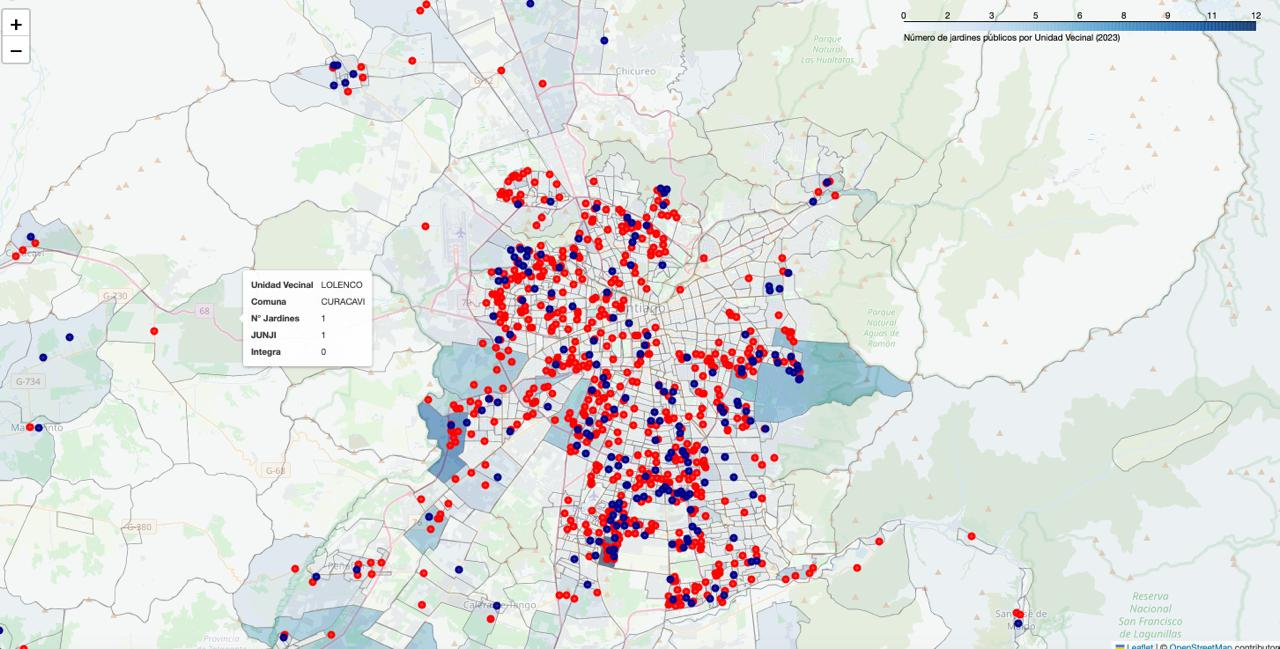
\includegraphics[width=\linewidth,height=0.62\textheight,keepaspectratio]{../jardines_uv_RM.jpeg}
\end{column}
\end{columns}
\fuente{Regi\'on Metropolitana. \textcolor{red}{$\bullet$} JUNJI \quad \textcolor{blue!60!black}{$\bullet$} Integra \quad Shading: public preschools per UV. Source: \texttt{base\_cobertura\_cp.dta}.}
\takeaway{One common geography: every preschool and every woman mapped to 2024 UV boundaries.}
\hfill\href{run:../output/figures/mapa_animado_rm.html}{\beamergotobutton{Interactive map 2014--2024}}
\end{frame}

\begin{frame}{Appendix A18. Examples of treated UVs}
\vspace{2pt}
\begin{columns}[T]
\begin{column}{0.5\textwidth}
\centering
{\small\textbf{\textcolor{navy}{Regi\'on Metropolitana}}}\\[2pt]
\includegraphics[width=0.98\textwidth,height=0.70\textheight,keepaspectratio]{../output/figures/mapa_uv_tratadas_panel.png}
\end{column}
\begin{column}{0.5\textwidth}
\centering
{\small\textbf{\textcolor{navy}{Valpara\'iso}}}\\[2pt]
\includegraphics[width=0.98\textwidth,height=0.70\textheight,keepaspectratio]{../output/figures/mapa_uv_tratadas_valparaiso.png}
\end{column}
\end{columns}
\fuente{Illustrative examples. Shaded: treated UVs (0 $\to$ 1+ preschools), 2015--2024.}
\end{frame}

% =============================================================================
% PREVIOUS RESULTS (before the October data fixes)
% =============================================================================
\begin{frame}[plain]
\vspace{50pt}
\begin{center}
{\LARGE\bfseries\color{navy} Previous results}\\[8pt]
{\large\color{graytext} Slides from the October 15 and 22 meetings, before the data fixes}
\end{center}
\end{frame}


% =============================================================================
% 10. WHO IS IN EACH SAMPLE AND WHAT WE MEASURE
% =============================================================================
\begin{frame}{Who is in each sample, and what we measure}
\begin{columns}[T]
\begin{column}{0.48\textwidth}
{\small\textcolor{steel}{\textbf{1. Samples}} \textcolor{graytext}{(selected at the individual level)}}
\begin{itemize}
  \small
  \item \textbf{Fertility}: women of fertile age (18--49)
  \item \textbf{Labor market}: women with a child $<$5 \emph{that specific year} --- not ``ever had a child''
  \item \textbf{First stage}: children of treatment-sample mothers, birth to birth+4
\end{itemize}
\end{column}
\begin{column}{0.48\textwidth}
{\small\textcolor{steel}{\textbf{2. Outcomes}} \textcolor{graytext}{(averaged at UV $\times$ year)}}
\begin{itemize}
  \small
  \item \textbf{Fertility}: share of women who had a child that year (Civil Registry birth records)
  \item \textbf{Labor market}: average annual income, months worked, share employed, dependent vs.\ independent
  \item \textbf{First stage}: enrollment rate
\end{itemize}
\end{column}
\end{columns}

\vspace{8pt}

\takeaway{Each outcome is measured on its relevant population, from administrative records, averaged at the UV $\times$ year level.}
\end{frame}

% =============================================================================
% 11. BALANCE EVIDENCE
% =============================================================================
\begin{frame}{Treated and never-treated UVs look alike --- except in size}
\noindent{\small\textcolor{steel}{\textbf{Labor market sample}} \textcolor{graytext}{(mothers with a child $<$5) --- covariate levels in 2014, before any opening}}\par
\vspace{2pt}
\begin{center}
\scriptsize
\renewcommand{\arraystretch}{0.95}
\setlength{\tabcolsep}{5pt}
\begin{tabular}{@{}lrrrrrrc@{}}
\toprule
 & \multicolumn{3}{c}{Unweighted} & \multicolumn{3}{c}{Weighted by UV population} & \\
\cmidrule(lr){2-4} \cmidrule(lr){5-7}
Variable & Never-tr. & Treated & Norm.\ diff. & Never-tr. & Treated & Norm.\ diff. & Sig.\textsuperscript{a} \\
\midrule
Formal employment (share) & 0.47 & 0.48 & 0.075 & 0.52 & 0.51 & -0.021 & -- \\
Annual income (M CLP) & 3.60 & 3.55 & -0.033 & 3.95 & 3.89 & -0.039 & * \\
Months worked         & 8.14 & 8.10 & -0.024 & 8.44 & 8.37 & -0.058 & * \\
Age                   & 29.24 & 29.25 & 0.008 & 29.26 & 29.29 & 0.026 & \\
N.\ children $<$5     & 1.11 & 1.11 & 0.045 & 1.11 & 1.11 & 0.049 & \\
Hours worked          & 37.07 & 37.68 & 0.099 & 36.55 & 36.81 & 0.068 & \\
Works (share)         & 0.45 & 0.45 & 0.023 & 0.48 & 0.48 & -0.006 & \\
Education (code)      & 4.98 & 5.02 & 0.028 & 5.20 & 5.18 & -0.020 & \\
\textbf{UV population} & 1126.79 & 2011.08 & \textbf{0.410} & 3530.92 & 5287.26 & \textbf{0.340} & *** \\
Child density 0--5 UV & 0.06 & 0.06 & 0.155 & 0.06 & 0.06 & 0.139 & *** \\
\midrule
N (UVs) & \multicolumn{2}{c}{3{,}909 \ / \ 422} & & \multicolumn{2}{c}{3{,}909 \ / \ 422} & & \\
\bottomrule
\end{tabular}
\end{center}
\vspace{-6pt}
{\tiny \textsuperscript{a} t-test at the woman level (* p$<$0.05, *** p$<$0.01), for reference only; normalized differences prioritized (concern threshold: 0.25); not computed for formal employment (--).}

\vspace{1pt}
{\footnotesize The UV population gap is \textbf{expected}: the State prioritizes new preschools where need and population are larger. Same pattern in the fertility sample (App.\ A4).}
\takeaway{Selection is in \emph{where} preschools open (UV size), not in \emph{who} lives there $\to$ UV fixed effects.}
\end{frame}

% =============================================================================
% 11b. MOVERS
% =============================================================================
\begin{frame}{About 1 in 3 mothers moves across UVs --- equally in treated and control UVs}
\begin{columns}[T]
\begin{column}{0.48\textwidth}
{\small\textcolor{steel}{\textbf{How many move?}}}
\begin{itemize}
  \footnotesize
  \item \textbf{33\%} of mothers change UV at least once while in the sample
  \item \textbf{7--12\% per year}
  \item \textbf{2022: 27\%} --- the year codes were standardized: likely an artifact, not real moves
\end{itemize}
\end{column}
\begin{column}{0.48\textwidth}
{\small\textcolor{steel}{\textbf{Do they move toward new preschools?}}}
\vspace{4pt}
\begin{center}
\footnotesize
\begin{tabular}{@{}lr@{}}
\toprule
Group & Moves (\% of mother-years) \\
\midrule
Treated & 12.6 \\
Never-treated & 12.3 \\
Excluded & 11.9 \\
\bottomrule
\end{tabular}
\end{center}
\end{column}
\end{columns}

\vspace{6pt}
\colorbox{bgpanel}{\parbox{0.97\linewidth}{\raggedright\footnotesize
\textbf{How we assign a UV to each woman}: RSH UV codes are not consistent across years; they are standardized only from 2022. For 2017--2021 we decoded them backwards by following the same women to the next year (majority rule) to place everyone on 2024 boundaries. $\to$ \textbf{Part of the measured moves may be decoding errors, not real moves} (e.g., the 2022 jump).}}

\vspace{3pt}
{\footnotesize Real moves dilute UV-level effects $\to$ we also follow each mother from her first UV (woman fixed effects, below).}
\takeaway{Mothers move often, but not toward UVs that open a preschool.}
\par\fuente{Moves measured with 2024 UV boundaries, the same map that defines treatment. Year-to-year changes from 2017 on (2014--2015 UVs are proxied by 2016). 33\% = among mothers observed in at least two comparable years.}
\end{frame}

% =============================================================================
% 11c. RESULTS -- BASELINE SPECIFICATION
% =============================================================================
\begin{frame}{Results: baseline specification}
\begin{block}{Results in the next slides use the previous definitions}
\footnotesize
\begin{itemize}
  \item \textbf{All women} in the RSH --- no vulnerability restriction
  \item \textbf{Labor market}: mothers with a child $<$5 \emph{that specific year}
  \item \textbf{First stage}: children of those mothers; \textbf{fertility}: women aged 18--49
  \item UV-level estimates, all treatment cohorts (2015 included)
\end{itemize}
\end{block}
\vspace{4pt}
\begin{block}{Suggestions from the last meeting}
\footnotesize
\begin{itemize}
  \item 60\% most vulnerable, mothers followed over time, individual-level estimates
  \item \textbf{Incorporated from slide~\ref{changes} on}
\end{itemize}
\end{block}
\takeaway{First the baseline results, then what changes with the new samples.}
\end{frame}

% =============================================================================
% 12. FIRST STAGE -- EVENT STUDY
% =============================================================================
\begin{frame}[label=fses]{First stage: enrollment rises the year a preschool opens and stays higher}
\begin{columns}[c]
\begin{column}{0.58\textwidth}
\centering
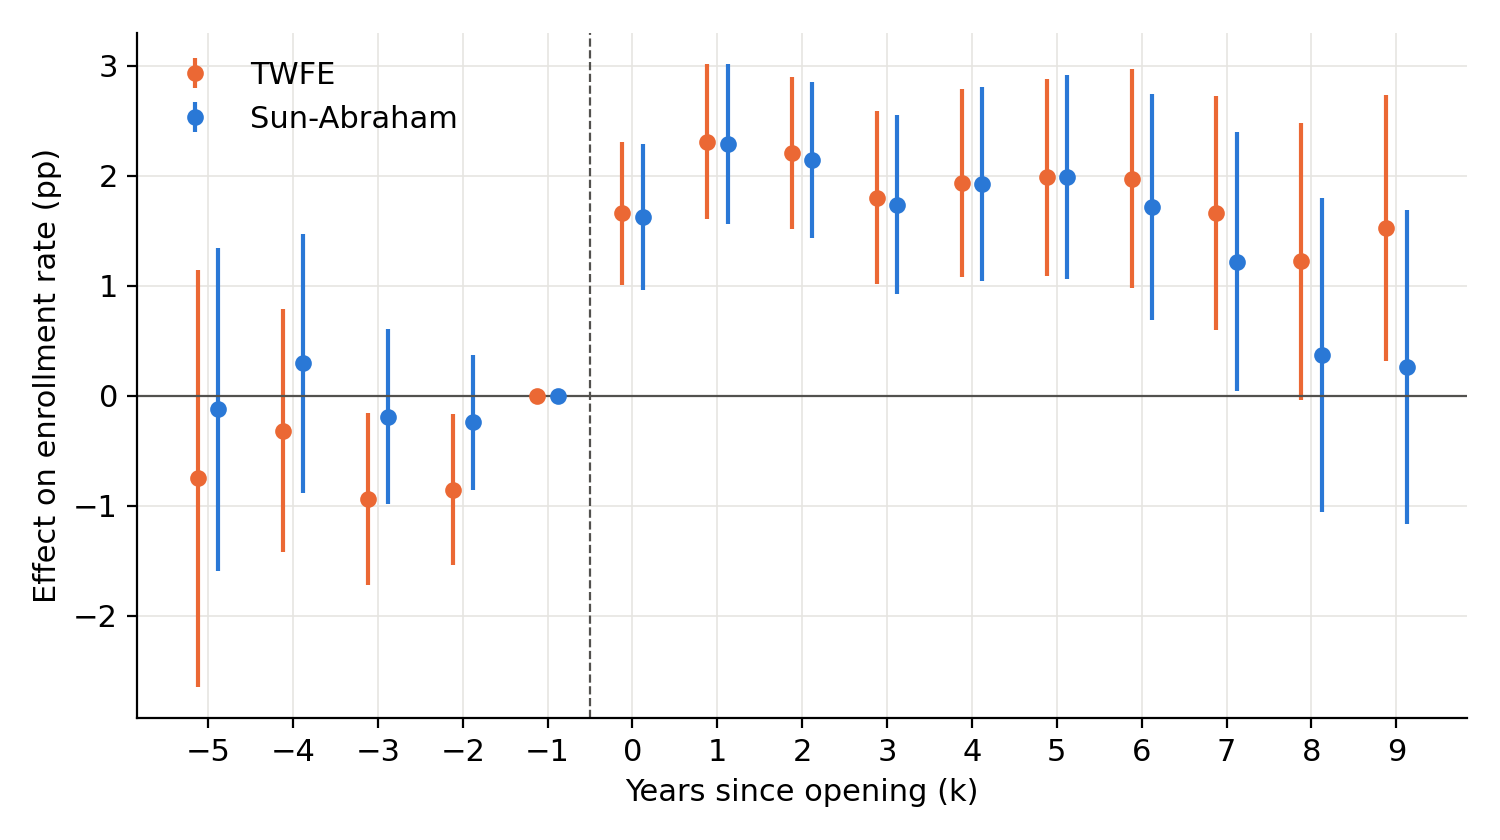
\includegraphics[width=\linewidth,height=0.62\textheight,keepaspectratio]{../RIS/20261006/graficos/pe_02_w_en.png}
\end{column}
\begin{column}{0.40\textwidth}
\begin{itemize}
  \footnotesize
  \item \textbf{Y-axis}: change in the enrollment rate (\% of children 0--4) in treated vs.\ never-treated UVs, relative to the year before opening
  \item Treated UVs: \textbf{33\% $\to$ $\approx$35\%} (+2pp), from the opening year on
  \item A treated UV has $\approx$\textbf{135 children} aged 0--4 $\to$ $\approx$\textbf{3 more enrolled}
  \item \textbf{No pre-trends}
  \item $k=7$--9: only early cohorts (mostly 2015) $\to$ composition, not a fading effect
\end{itemize}

\end{column}
\end{columns}
\takeaway{A new preschool raises enrollment from 33\% to $\approx$35\%: $\approx$3 more children per UV.}
\par\fuente{Weighted by number of children. Sun--Abraham and TWFE, 95\% CI clustered by UV. Children aged 0--4.}
\end{frame}

% =============================================================================
% 14. FIRST STAGE -- BY CHILD AGE
% =============================================================================
\begin{frame}{First stage by child age: strongest at ages 2--3}
\centering
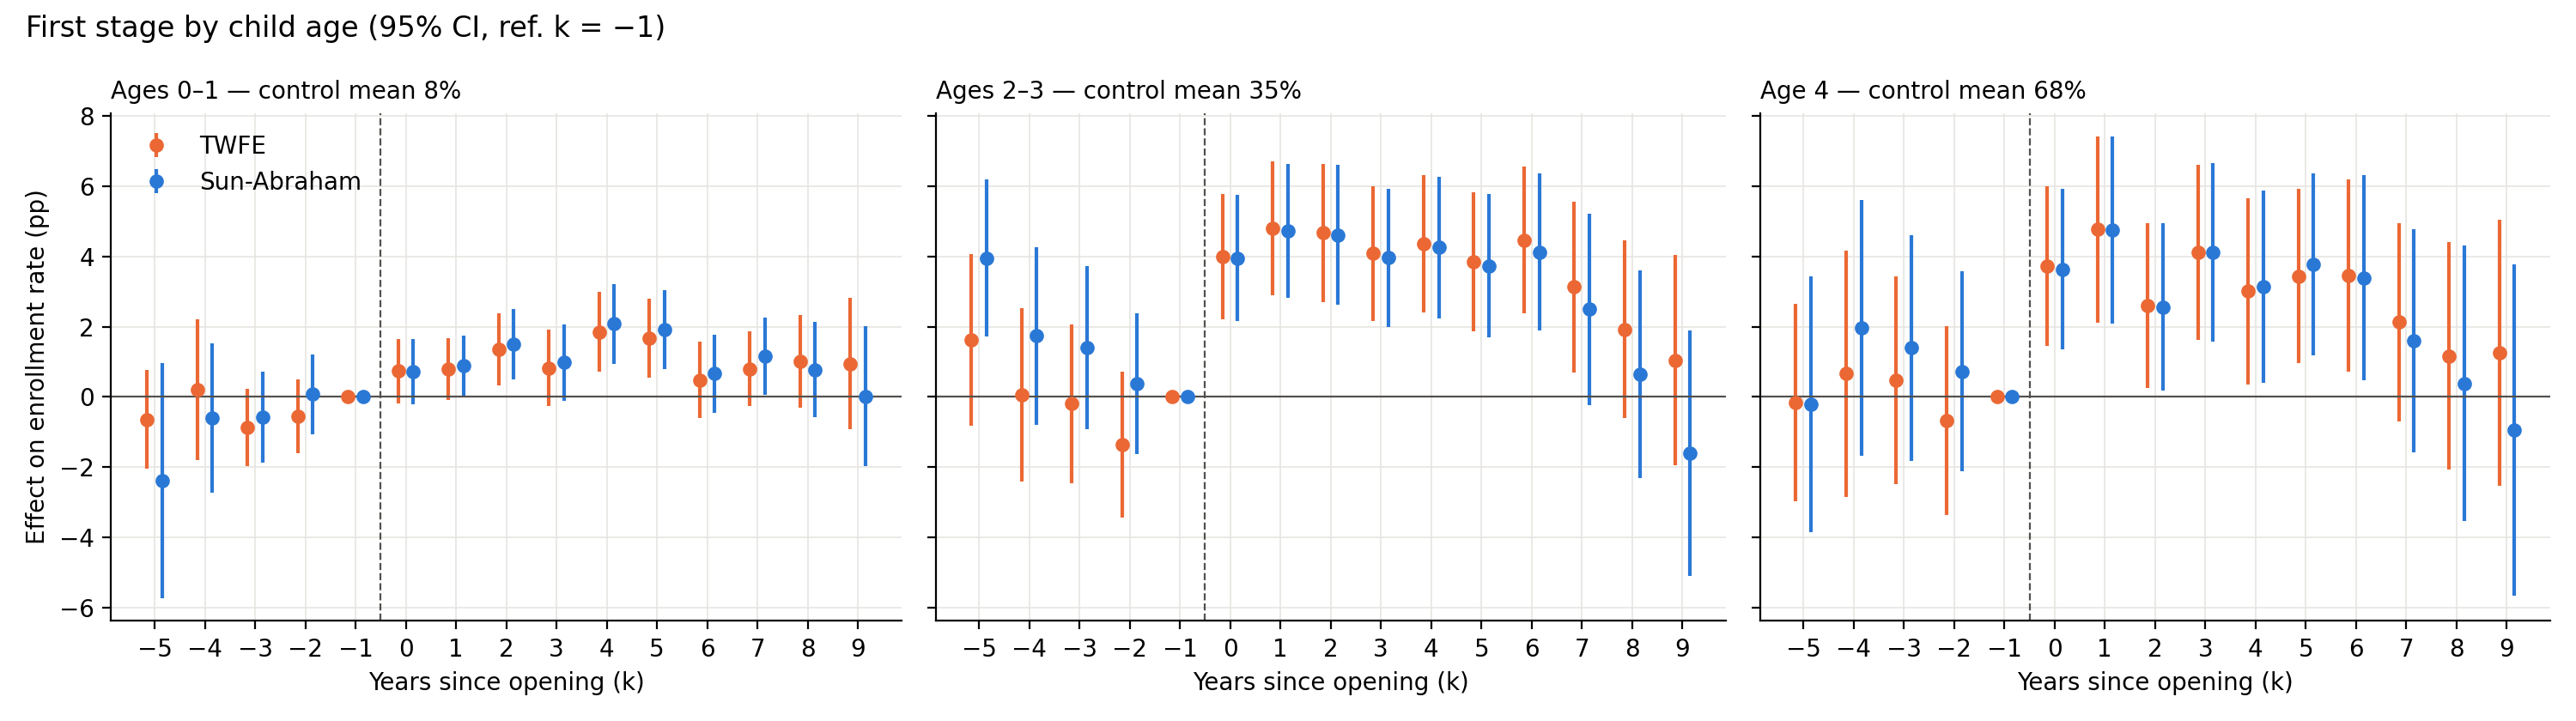
\includegraphics[width=\linewidth,height=0.42\textheight,keepaspectratio]{../RIS/20261006/graficos/pe_03_het_edad_en.png}

\vspace{4pt}
\begin{columns}[T]
\begin{column}{0.50\textwidth}
\scriptsize
\setlength{\tabcolsep}{4pt}
\begin{tabular}{@{}lrrr@{}}
\toprule
Child age & Control mean & SA $k=0$--6 & Relative \\
\midrule
Ages 0--1 & 8\% & +1.3pp & +15\% \\
\textbf{Ages 2--3} & 35\% & \textbf{+4.2pp} & +12\% \\
Age 4 & 68\% & +3.6pp & +5\% \\
\bottomrule
\end{tabular}
\end{column}
\begin{column}{0.46\textwidth}
\begin{itemize}
  \footnotesize
  \item \textbf{Ages 2--3}: largest effect, immediate and stable
  \item \textbf{Ages 0--1}: small in pp but largest in relative terms; grows over time
  \item \textbf{Age 4}: also positive
  \item \textbf{Caution}: ages are measured at different points in time across datasets (to check)
\end{itemize}
\end{column}
\end{columns}
\raggedright\takeaway{Enrollment rises at all ages, most at ages 2--3.}
\end{frame}

% =============================================================================
% 15. THE 2015 COHORT
% =============================================================================
\begin{frame}{An open issue: the 2015 cohort}
\centering
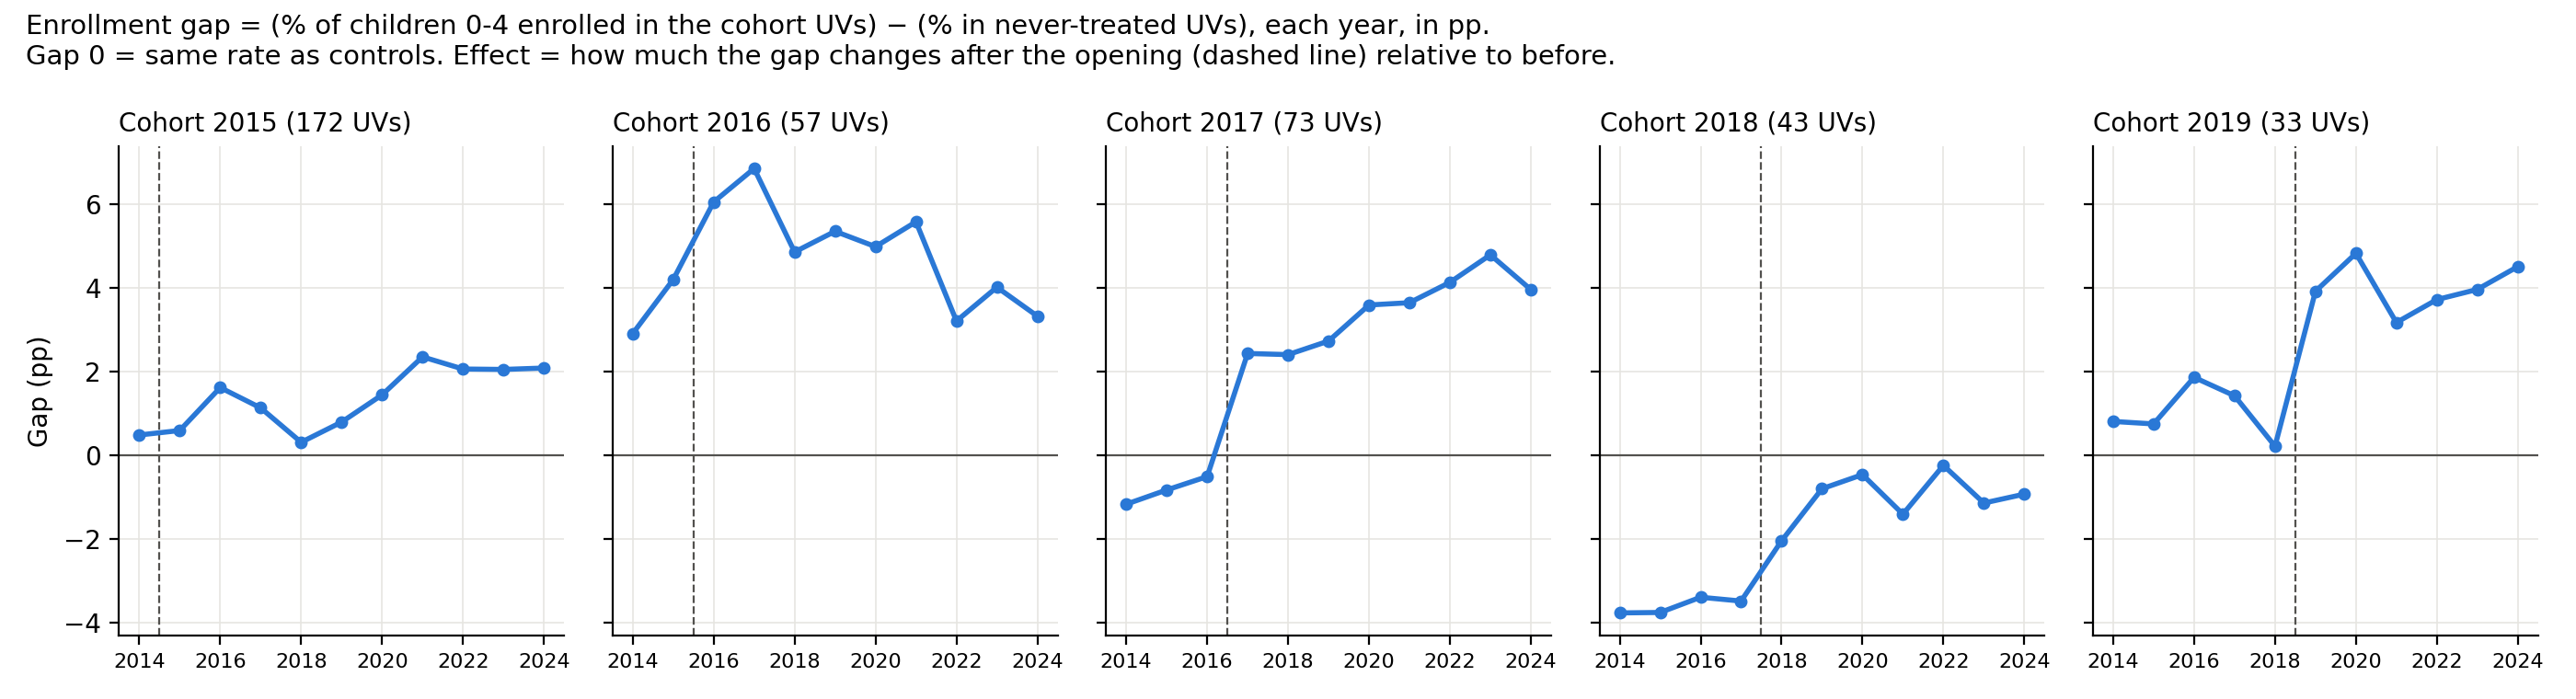
\includegraphics[width=\linewidth,height=0.38\textheight,keepaspectratio]{../RIS/20261006/graficos/pe_01b_brecha_cohortes_en.png}

\vspace{2pt}
\begin{columns}[T]
\begin{column}{0.52\textwidth}
\begin{itemize}
  \footnotesize
  \item \textbf{172 UVs} --- 41\% of treated UVs, $\sim$half of the sample at $k=6$, the only cohort at $k=9$
  \item Its effect is \textbf{very small} ($\approx$0.7pp in raw gaps) and it has only one pre-period (2014)
\end{itemize}
\end{column}
\begin{column}{0.46\textwidth}
\colorbox{bgpanel}{\parbox{0.95\linewidth}{\raggedright\footnotesize
\textbf{Hypothesis}: registration error at the edge of the panel --- preschools that already operated in 2014 but are recorded as 2015 openings.\\[2pt]
\textbf{Next}: carefully review the coverage data provided by JUNJI/Integra.}}
\end{column}
\end{columns}
\takeaway{The 2015 cohort pulls the average effect down --- possibly a data error to check.}
\end{frame}

% =============================================================================
% 23. FIRST STAGE WITHOUT 2015
% =============================================================================
\begin{frame}[label=fs15]{Without the 2015 cohort, the first stage is $\sim$50\% larger}
\begin{columns}[c]
\begin{column}{0.58\textwidth}
\centering
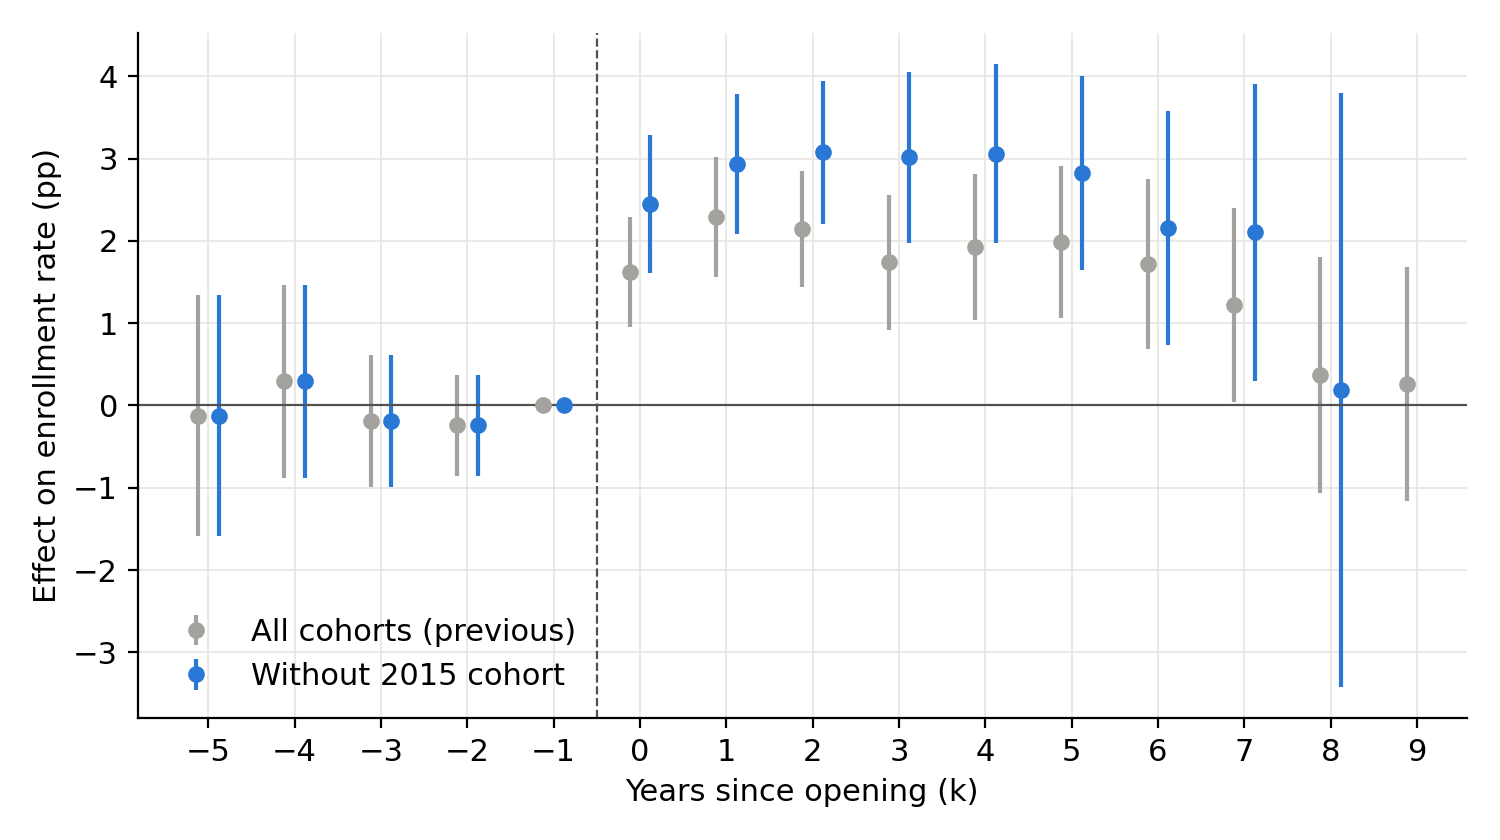
\includegraphics[width=\linewidth,height=0.62\textheight,keepaspectratio]{../RIS/20261014/graficos/en_pe_sin2015.png}
\end{column}
\begin{column}{0.40\textwidth}
\begin{itemize}
  \footnotesize
  \item Same pre-periods (the 2015 cohort has none)
  \item \textbf{+2.7pp} vs.\ +1.8pp: $\approx$\textbf{4 more children} enrolled per UV instead of 3
  \item Jumps at opening and stays stable
  \item Earnings: the effect also roughly doubles without 2015
\end{itemize}
\end{column}
\end{columns}
\takeaway{The 2015 cohort dilutes the first stage --- but it remains small.}
\par\fuente{All mothers (first stage not yet estimated for the 60\% most vulnerable). Average $k=0$--7. Sun--Abraham, weighted by number of children, 95\% CI clustered by UV.}
\end{frame}


% =============================================================================
% 16. CLEAN CONTROL -- MOTIVATION
% =============================================================================
\begin{frame}{A cleaner control group: never-treated UVs can be exposed too}
\begin{columns}[c]
\begin{column}{0.40\textwidth}
\begin{itemize}
  \footnotesize
  \item \textbf{Concern}: children from a never-treated UV can enroll in a new preschool next door $\to$ control enrollment rises $\to$ \textbf{effect underestimated}
  \item We built a \textbf{neighbor map}: for every UV, which adjacent UVs had or opened a preschool (shared border, 2024 boundaries)
  \item Example: this control UV has 9 neighbors --- \textbf{5 open a preschool} during the period
\end{itemize}
\end{column}
\begin{column}{0.58\textwidth}
\centering
\includegraphics[width=\linewidth,height=0.72\textheight,keepaspectratio]{../output/figures/spillover_1_ejemplo_uv_en.png}
\end{column}
\end{columns}
\takeaway{Goal: a larger first stage, comparing treated UVs with controls that could \emph{not} use a neighbor's new preschool.}
\par\fuente{* Neighbors only capture proximity to home. If mothers use preschools near their workplace, spillovers may reach UVs that are not adjacent.}
\end{frame}

% =============================================================================
% 17. CLEAN CONTROL -- RESULTS
% =============================================================================
\begin{frame}{A cleaner control group gives the same first stage}
\centering
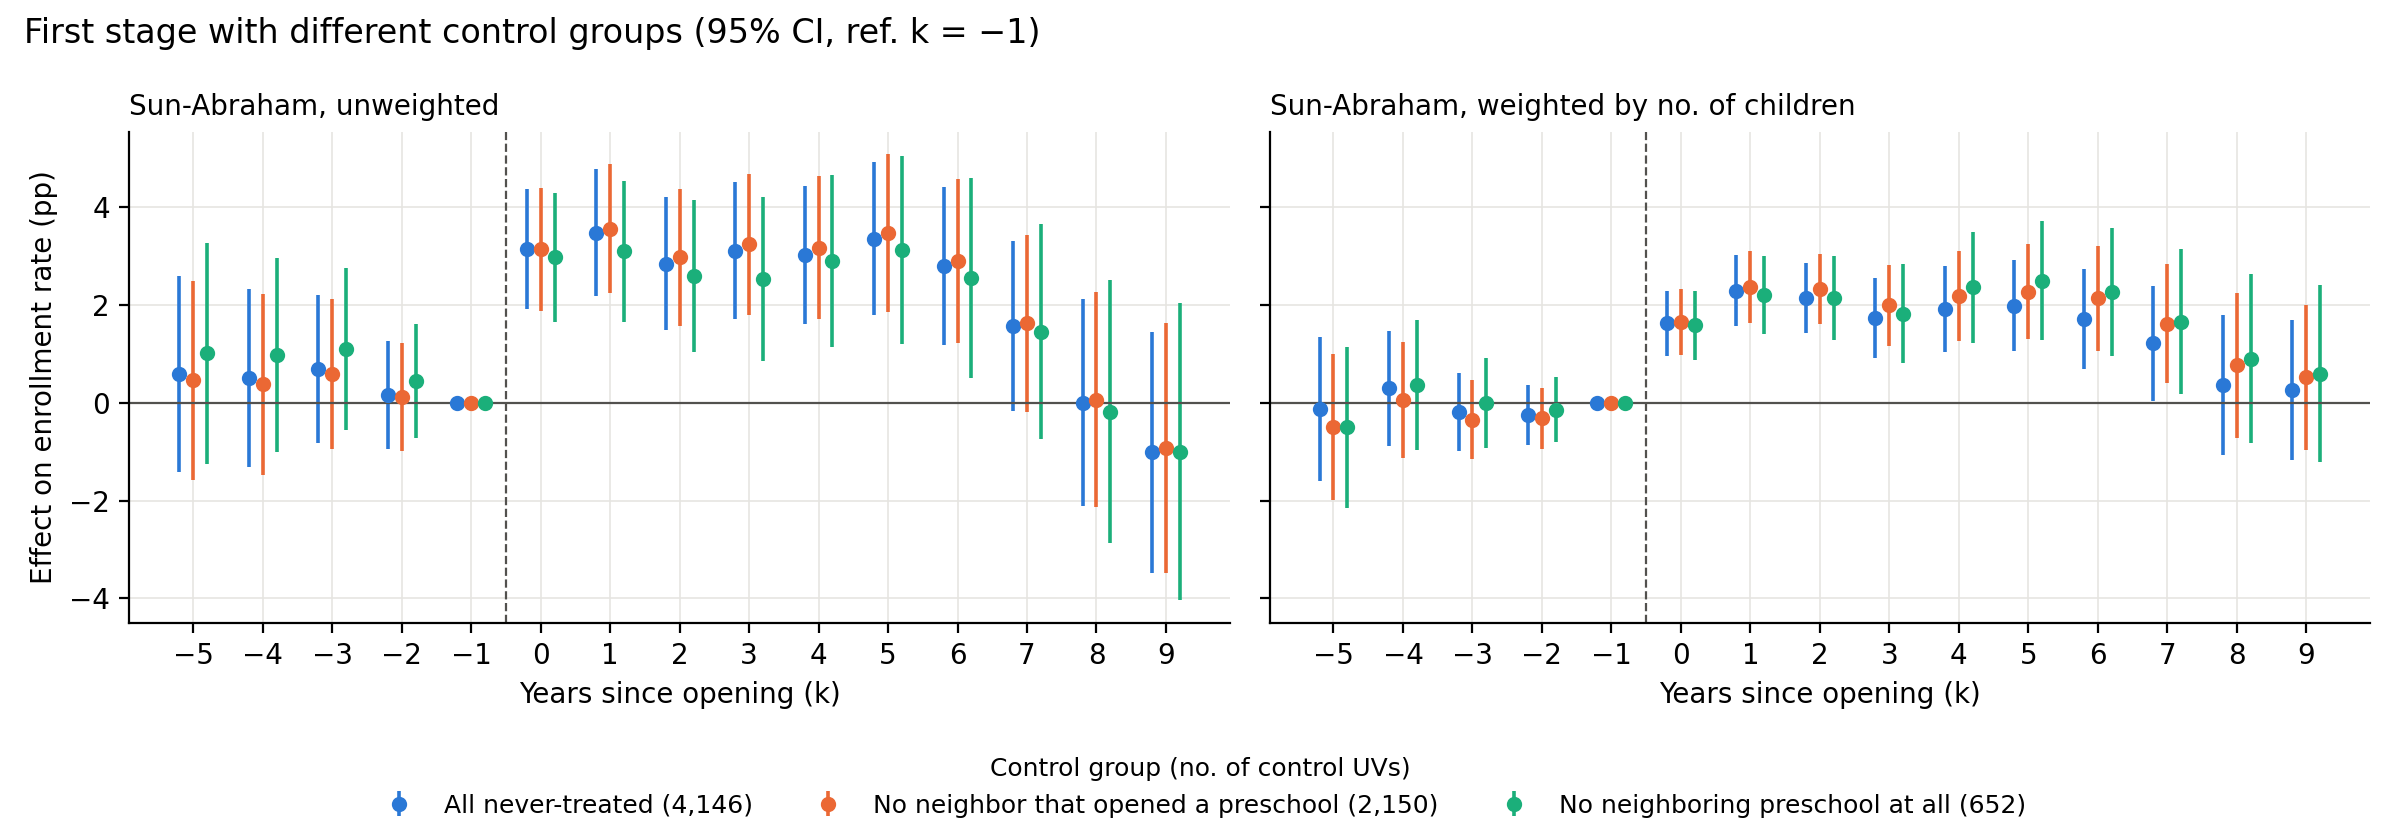
\includegraphics[width=0.92\linewidth,height=0.36\textheight,keepaspectratio]{../RIS/20261006/graficos/pe_04_control_limpio_en.png}

\vspace{2pt}
\scriptsize
\begin{tabular}{@{}lrrrr@{}}
\toprule
Control group & UVs & Median area & Control mean & SA weighted, $k=0$--6 \\
\midrule
All never-treated (main) & 4{,}146 & 2.8 km$^2$ & 33.2\% & 1.92 \\
\textbf{No neighbor opened a preschool 2015--24} & \textbf{2{,}150} & 3.8 km$^2$ & 32.7\% & \textbf{2.14} \\
No neighboring preschool in any year & 652 & \textbf{6.7 km$^2$} & 28.2\% & 2.13 \\
\midrule
\textit{Treated UVs} & \textit{422} & \textit{1.5 km$^2$} & & \\
\bottomrule
\end{tabular}

\raggedright
\vspace{3pt}
\footnotesize Same effect with all three groups and clean pre-trends. The strictest group is not a good comparison: its UVs are \textbf{$\sim$4$\times$ larger} than treated ones (isolated areas) $\to$ preferred clean control: \textbf{no neighbor opened}.
\takeaway{Spillovers to controls do not explain the small first stage.}
\end{frame}

% =============================================================================
% 18b. WHY IS THE FIRST STAGE SMALL?
% =============================================================================
\begin{frame}{Why is the first stage small?}
\begin{columns}[T]
\begin{column}{0.44\textwidth}
{\small\textcolor{steel}{\textbf{What we checked}}}
\begin{itemize}
  \footnotesize
  \item \textbf{2015 cohort}: very small effect, possibly a data error $\to$ without it, $\approx$3pp
  \item \textbf{Cleaner control group}: same $\approx$2pp $\to$ spillovers to controls are not the reason
\end{itemize}

\vspace{6pt}
{\small\textcolor{steel}{\textbf{What our outcome measures}}}
\begin{itemize}
  \footnotesize
  \item Whether children \textbf{living} in the treated UV are enrolled in \textbf{any} preschool
\end{itemize}
\end{column}
\begin{column}{0.54\textwidth}
{\small\textcolor{steel}{\textbf{A new preschool can fill up without moving our outcome}}}
\begin{itemize}
  \footnotesize
  \item It raises enrollment only if it takes local children who were \textbf{not enrolled before}
  \item \textbf{Substitution}: local children already enrolled elsewhere switch to the new preschool $\to$ no net change
  \item \textbf{Mothers use other preschools}, e.g.\ near their workplace in another UV $\to$ new places go to children from other UVs
\end{itemize}

\vspace{6pt}
\colorbox{bgpanel}{\parbox{0.95\linewidth}{\raggedright\footnotesize
\textbf{Future work}: enrollment records show which preschool each child attends $\to$ who fills the new preschool, where they live, and which preschools local mothers use.}}
\end{column}
\end{columns}
\takeaway{Enrollment of local children can move little, even if the new preschool fills up.}
\end{frame}

% =============================================================================
% 18. FERTILITY
% =============================================================================
\begin{frame}{Fertility: no effect yet}
\centering
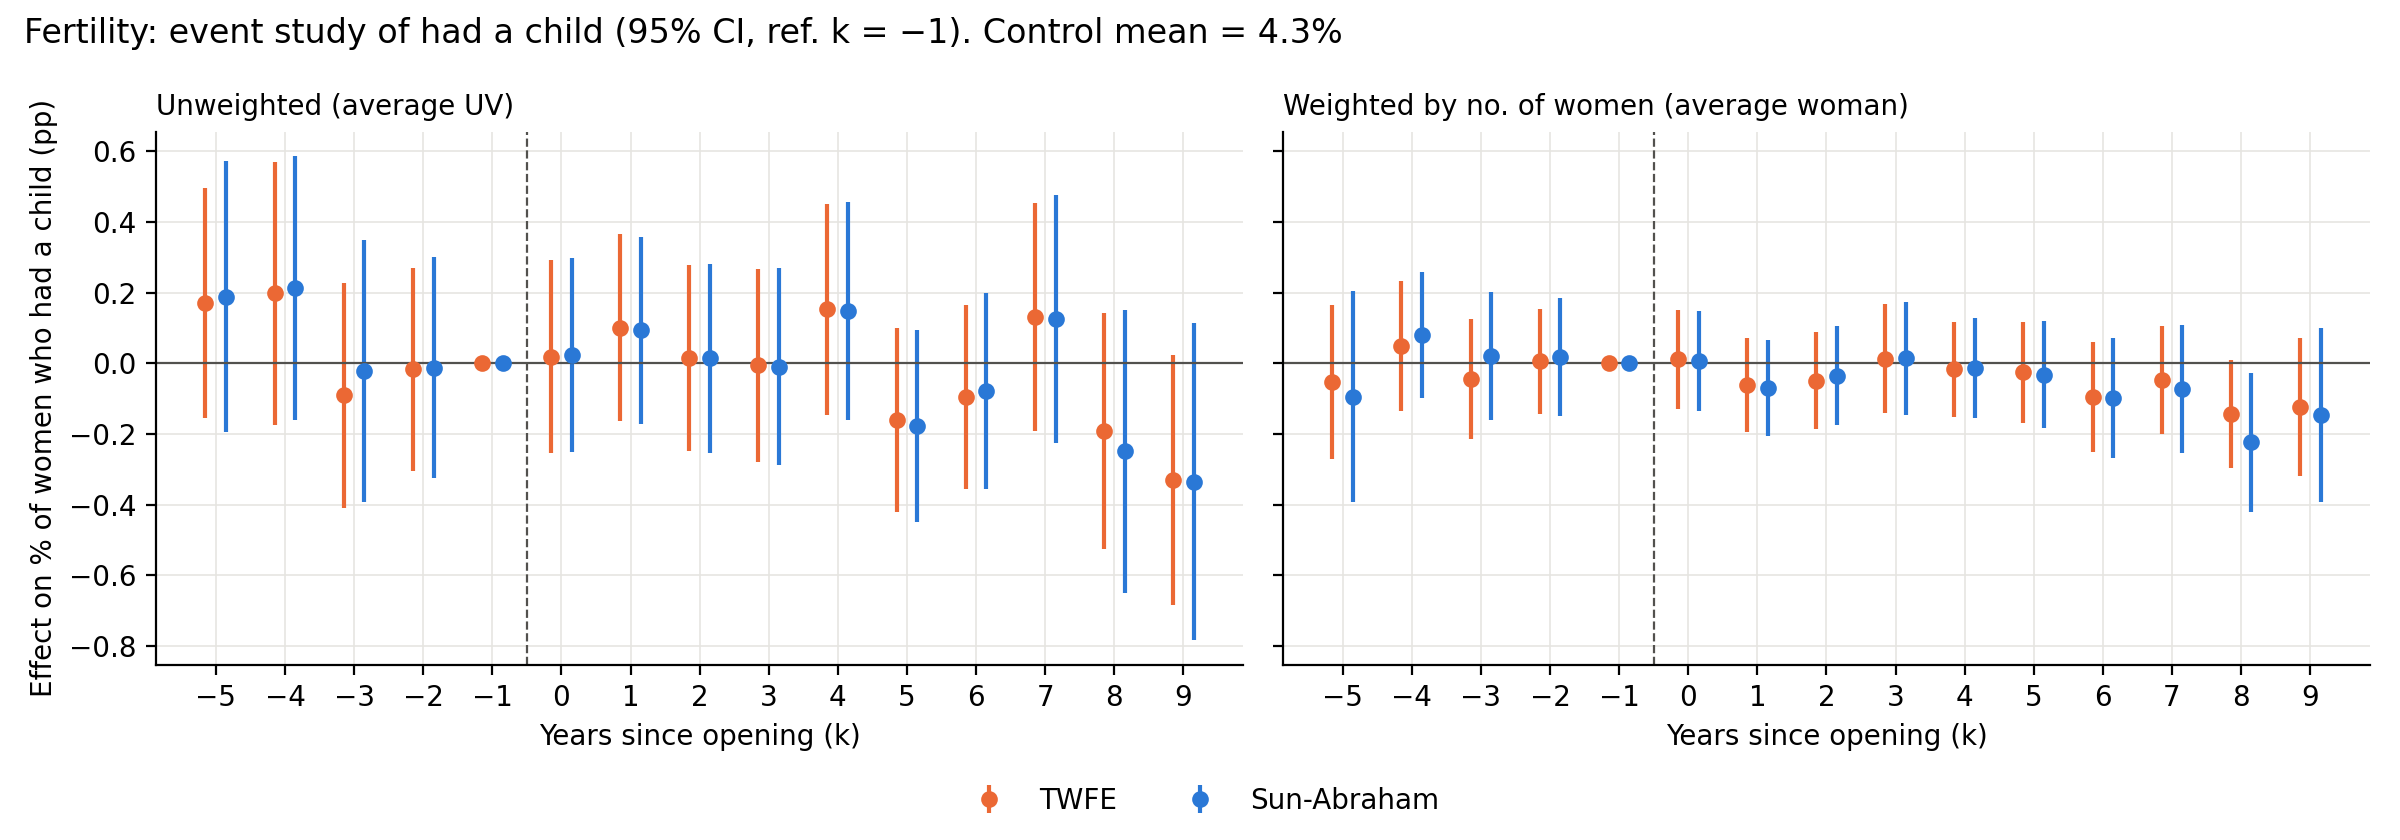
\includegraphics[width=\linewidth,height=0.50\textheight,keepaspectratio]{../RIS/20261006/graficos/fe_02_eventstudy_en.png}

\vspace{2pt}
\begin{columns}[T]
\begin{column}{0.50\textwidth}
\begin{itemize}
  \footnotesize
  \item Treated and control UVs decline together; \textbf{no jump at opening}
  \item Clean pre-trends
\end{itemize}
\end{column}
\begin{column}{0.48\textwidth}
\begin{itemize}
  \footnotesize
  \item A \textbf{fairly precise zero}: rules out large effects
  \item Still checking: cumulative outcome (having had a child)
\end{itemize}
\end{column}
\end{columns}
\raggedright\takeaway{Expected: having a child depends on many factors, and a nearby preschool might weigh little.}
\par\fuente{Women aged 18--49. Outcome: share who had a child in the year (control mean 4.3\%). Controls for average age.}
\end{frame}

% =============================================================================
% 19. FORMAL EMPLOYMENT
% =============================================================================
\begin{frame}{Mothers' formal employment rises by 1pp from the fourth year}
\begin{columns}[c]
\begin{column}{0.58\textwidth}
\centering
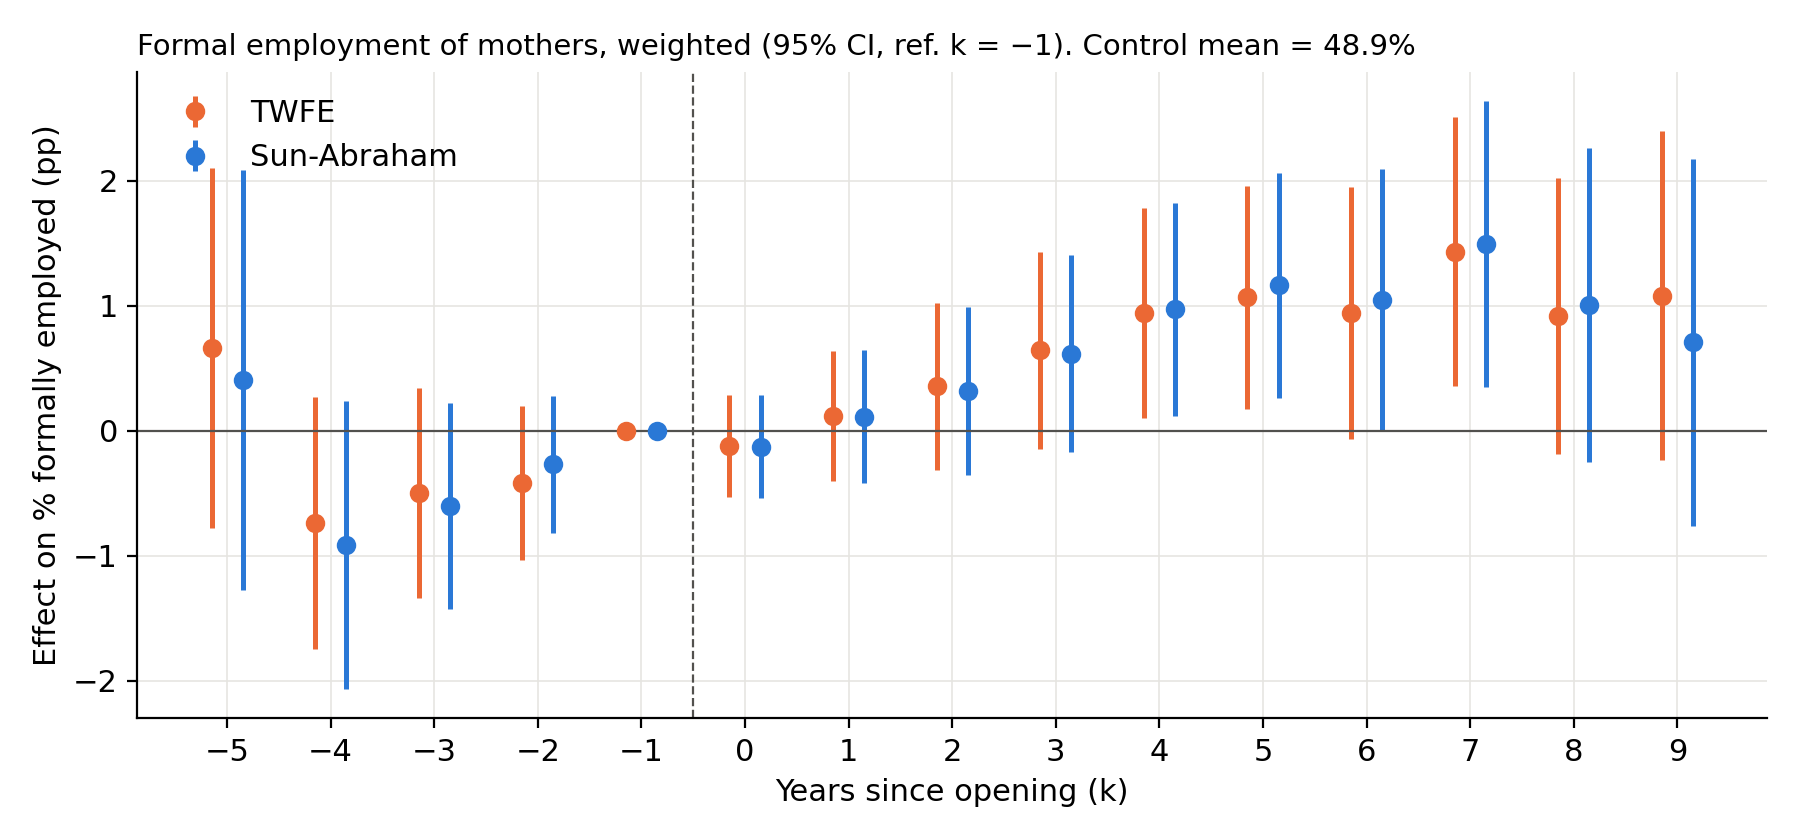
\includegraphics[width=\linewidth,height=0.62\textheight,keepaspectratio]{../RIS/20261006/graficos/lab_02a_empleo_w_en.png}
\end{column}
\begin{column}{0.40\textwidth}
\begin{itemize}
  \footnotesize
  \item Nothing at opening; \textbf{significant from $k=4$}; no pre-trends ($p=0.82$)
\end{itemize}

\vspace{2pt}
{\footnotesize\textcolor{steel}{\textbf{Why gradual? Two possible reasons}}}
\begin{itemize}
  \footnotesize
  \item \textbf{Who is in the sample}: if the child is already 3--4 at opening, the mother barely uses it; later, more mothers had it since birth
  \item \textbf{Returning to work takes time}
\end{itemize}
{\scriptsize How to tell them apart:}
\begin{itemize}
  \scriptsize
  \item Keep mothers until 2024 $\to$ no one leaves when her child turns 5
  \item Woman FE $\to$ each mother compared with herself
  \item If still gradual $\to$ it is the time to return to work
\end{itemize}

\end{column}
\end{columns}
\takeaway{A new preschool raises mothers' formal employment by $\approx$1pp from the fourth year.}
\par\fuente{Weighted by number of mothers. Mothers with a child $<$5 that year. Employed = any taxable income or contribution.}
\end{frame}

% =============================================================================
% 20. NEW THIS WEEK -- SAMPLE CHANGES
% =============================================================================
\begin{frame}[label=changes]{Changes to the samples}
\begin{block}{1. Only the 60\% most vulnerable (labor and fertility samples)}
\footnotesize
\begin{itemize}
  \item The population \textbf{eligible} for JUNJI/Integra preschools $\to$ removes women who could not be treated
  \item Vulnerable = RSH bracket $\leq$60 (FPS score $\leq$13{,}500 in 2014--2015, new samples only)
  \item \textbf{Fixed per woman}: her classification in the \textbf{first year she appears}, kept for all years $\to$ does not respond to the opening
\end{itemize}
\end{block}
\vspace{2pt}
\begin{block}{2. Mothers stay in the labor sample (in progress)}
\footnotesize
\begin{itemize}
  \item Before: a mother is in the sample only \textbf{while} she has a child $<$5
  \item Now: she enters the first year she has a child $<$5 and \textbf{stays until 2024}, even after the child turns 5 $\to$ the sample no longer changes with births and children aging out
\end{itemize}
\end{block}
\takeaway{We now focus on eligible mothers and follow the same mothers over time.}
\par\fuente{Results below: change 1 with RSH only and the previous mother definition. FPS and change 2: new samples being built.}
\end{frame}

% =============================================================================
% 20b. WHERE WE ARE
% =============================================================================
\begin{frame}{Where each change stands}
\begin{center}
\footnotesize
\renewcommand{\arraystretch}{1.35}
\begin{tabular}{@{}lccc@{}}
\toprule
 & \textbf{First stage} & \textbf{Labor market} & \textbf{Fertility} \\
\midrule
60\% most vulnerable & \textcolor{graytext}{pending} & \textbf{done} (slides \ref{empv}--\ref{ingv}) & \textcolor{graytext}{pending} \\
Mothers followed until 2024 & --- & \textcolor{graytext}{running} & --- \\
Woman FE, fixed UV & --- & \textbf{preliminary} (slide \ref{femuj}) & --- \\
Without the 2015 cohort & \textbf{done} (slide \ref{fs15}) & \textbf{done}: similar & \textcolor{graytext}{pending} \\
Earnings including zeros & --- & \textbf{done} (slide \ref{ingv}) & --- \\
\bottomrule
\end{tabular}
\end{center}
\vspace{4pt}
{\footnotesize Labor results for vulnerable mothers use RSH only and the previous mother definition. The first stage for their children comes next.}
\takeaway{Labor results already reflect the vulnerable sample; first stage and fertility come next.}
\end{frame}

% =============================================================================
% 21. EMPLOYMENT -- 60% MOST VULNERABLE
% =============================================================================
\begin{frame}[label=empv]{Employment: same effect among the 60\% most vulnerable}
\begin{columns}[c]
\begin{column}{0.58\textwidth}
\centering
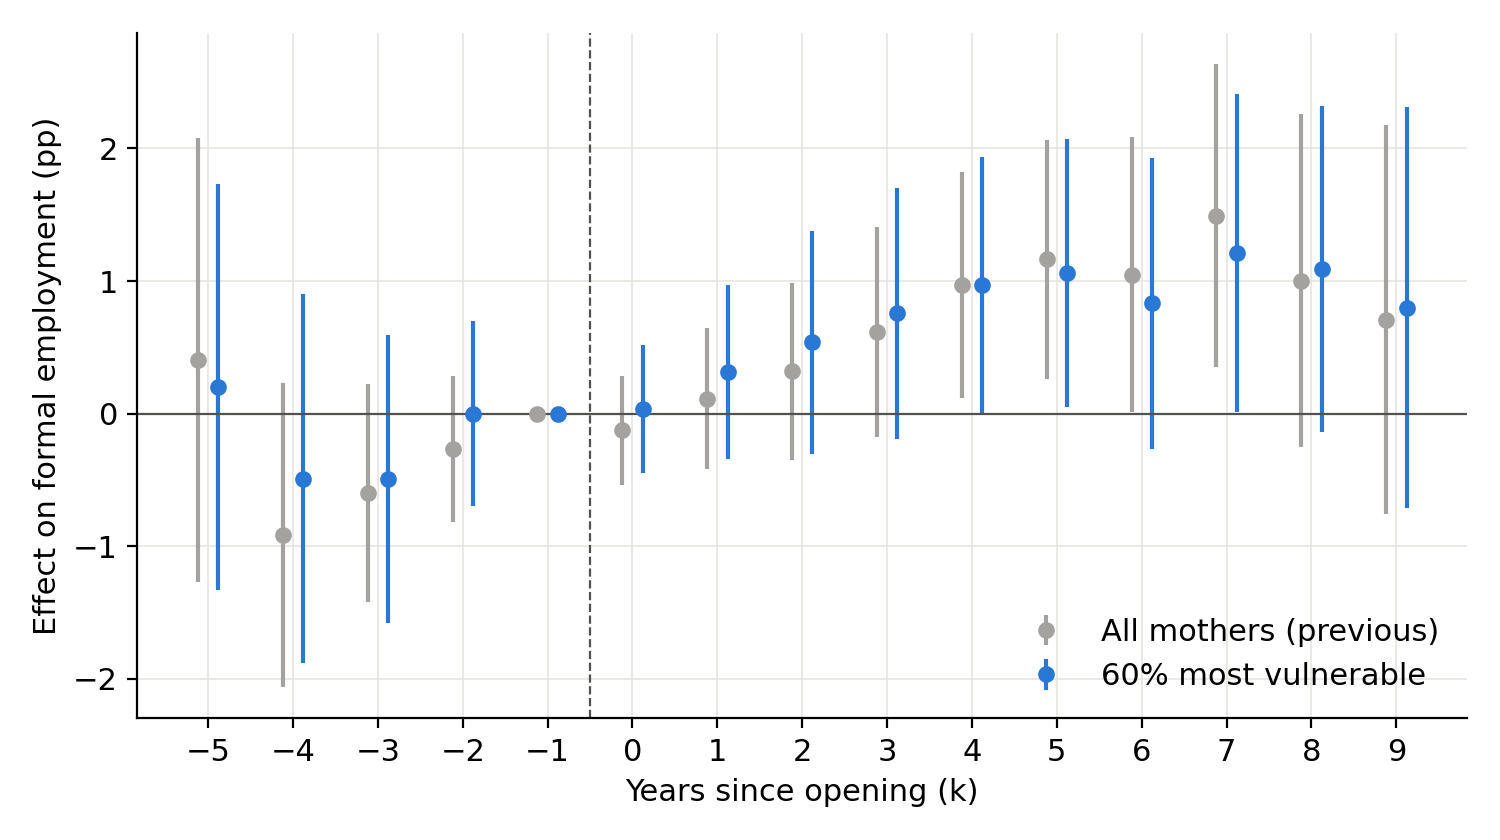
\includegraphics[width=\linewidth,height=0.62\textheight,keepaspectratio]{../RIS/20261014/graficos/en_v60_empleo.png}
\end{column}
\begin{column}{0.40\textwidth}
\begin{itemize}
  \footnotesize
  \item \textbf{No pre-trends} (joint test $p=0.79$)
  \item Gradual, $\approx$+1pp from the 4th year; average \textbf{+0.8pp} on a 46\% base ($\approx$+1.6\%), significant
\end{itemize}
\vspace{2pt}
\colorbox{bgpanel}{\parbox{0.95\linewidth}{\raggedright\scriptsize
\textbf{Why so similar to all mothers?} If the non-vulnerable third had no effect, we would expect $\approx$1.1pp (same effect, fewer mothers). But:
\begin{itemize}
  \item Those excluded are RSH middle class, not rich; vulnerable mothers are 2/3 of the sample
  \item Eligibility is not strict: free places go to other families
\end{itemize}
Next: estimate the non-vulnerable separately.}}
\end{column}
\end{columns}
\takeaway{The employment effect holds in the eligible population.}
\par\fuente{Sun--Abraham, weighted by number of mothers, 95\% CI clustered by UV, ref.\ $k=-1$.}
\end{frame}

% =============================================================================
% 22b. LN EARNINGS (WORKING MOTHERS)
% =============================================================================
\begin{frame}[label=lnv]{Working mothers do not earn more}
\begin{columns}[c]
\begin{column}{0.58\textwidth}
\centering
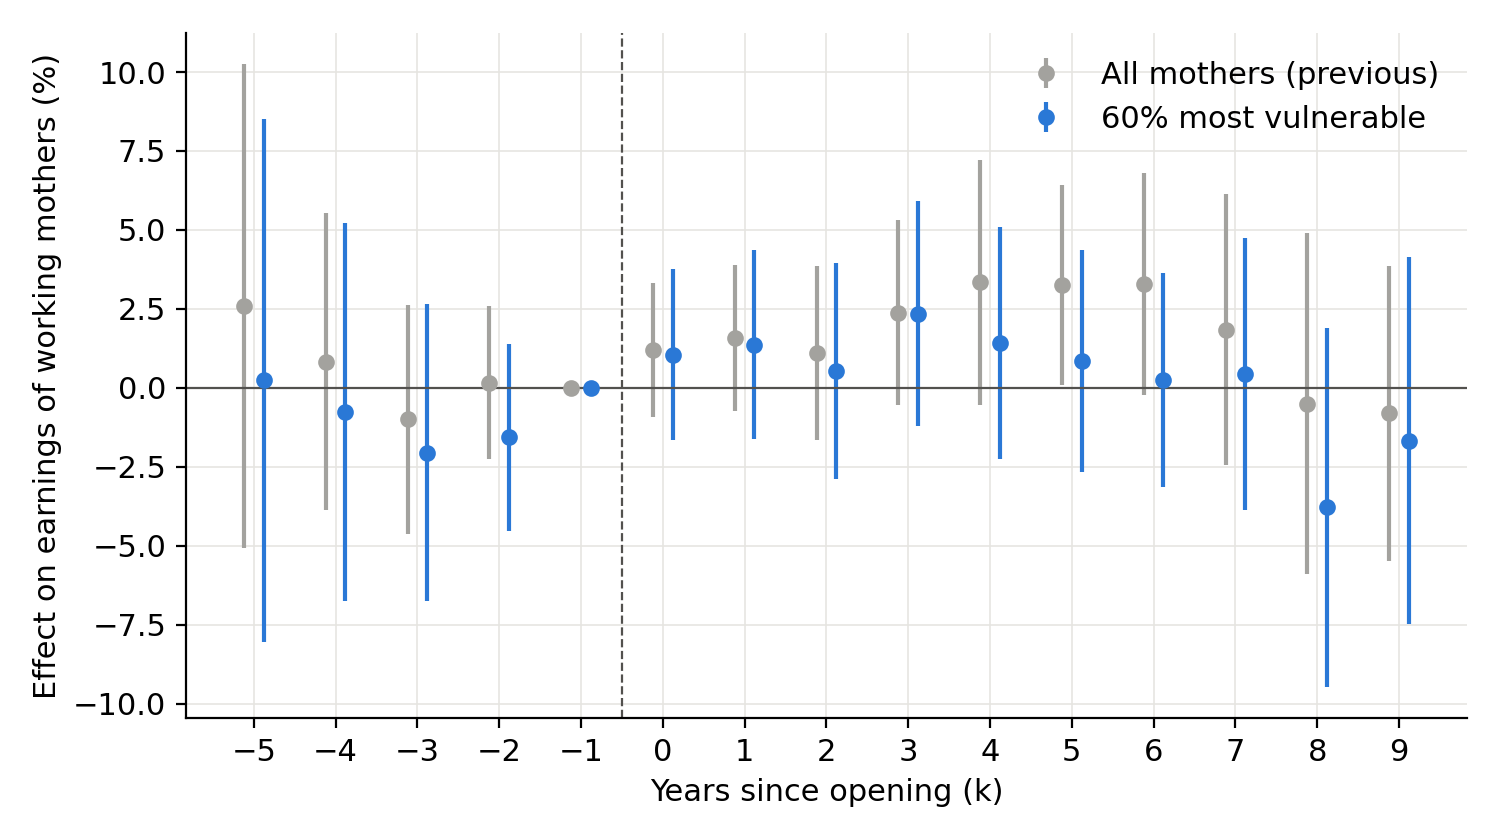
\includegraphics[width=\linewidth,height=0.62\textheight,keepaspectratio]{../RIS/20261014/graficos/en_v60_ln_ingreso.png}
\end{column}
\begin{column}{0.40\textwidth}
\begin{itemize}
  \footnotesize
  \item ln earnings: \textbf{only mothers who work}
  \item \textbf{No pre-trends}; after opening, $\approx$\textbf{0} among vulnerable mothers (+0.3\%, not significant)
  \item All mothers: slightly higher ($\approx$+3\% at $k=3$--6), also not significant
  \item Months worked: also no effect
\end{itemize}
\end{column}
\end{columns}
\takeaway{The earnings gain does not come from higher wages.}
\par\fuente{Sun--Abraham, weighted by number of mothers with earnings, 95\% CI clustered by UV, reference $k=-1$. Mothers with a child $<$5 that year.}
\end{frame}

% =============================================================================
% 22. EARNINGS INCLUDING ZEROS
% =============================================================================
\begin{frame}[label=ingv]{Earnings rise because more mothers work, not because they earn more}
\begin{columns}[c]
\begin{column}{0.58\textwidth}
\centering
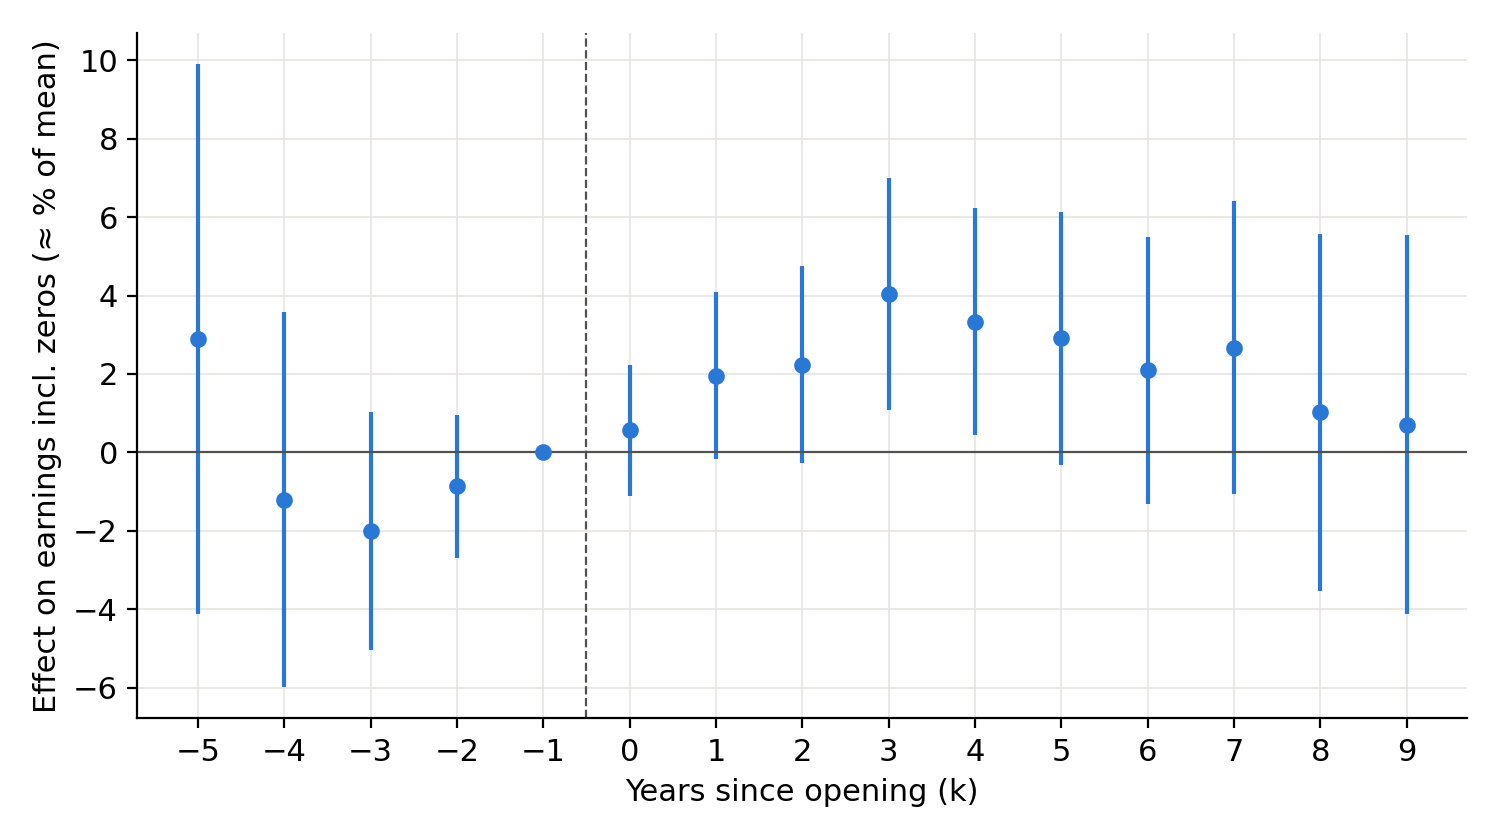
\includegraphics[width=\linewidth,height=0.62\textheight,keepaspectratio]{../RIS/20261014/graficos/en_v60_ingreso_rel.png}
\end{column}
\begin{column}{0.40\textwidth}
\begin{itemize}
  \footnotesize
  \item Earnings \textbf{including zeros}: average over \emph{all} mothers, those without earnings count as 0
  \item \textbf{Y-axis}: 100 = average mother that year $\to$ \textbf{+2 points $\approx$ +2\%}
  \item Average after opening: $\approx$\textbf{+2\%}, peak at $k=3$--4 (significant at 10\%)
  \item $\sim$\textbf{3/4} of it is explained by more mothers working
  \item Among mothers who work: earnings and months worked \textbf{do not change}
\end{itemize}
\end{column}
\end{columns}
\takeaway{The preschool changes \emph{whether} mothers work, not how much those already working earn.}
\par\fuente{60\% most vulnerable. Earnings relative to the year's mean (100). Sun--Abraham, weighted by number of mothers, 95\% CI clustered by UV.}
\end{frame}

% =============================================================================
% 24. WOMAN FIXED EFFECTS
% =============================================================================
\begin{frame}[label=femuj]{Woman fixed effects: a design to discuss}
\begin{columns}[T]
\begin{column}{0.49\textwidth}
{\small\textcolor{steel}{\textbf{Approach}}}
\begin{itemize}
  \footnotesize
  \item Compare \textbf{the same mother} before and after the opening $\to$ removes her fixed traits (e.g., attachment to work)
  \item Treatment from her \textbf{UV before the opening}, kept if she moves (intention-to-treat)
  \item Movers are \textbf{not dropped}: staying could itself respond to the preschool
\end{itemize}
\vspace{2pt}
{\small\textcolor{steel}{\textbf{Results so far} (preliminary)}}
\begin{itemize}
  \footnotesize
  \item Employment: no pre-trends; gradual, significant from the 4th year, $\approx$+1.6pp by $k=9$ --- same pattern as UV level
\end{itemize}
\end{column}
\begin{column}{0.49\textwidth}
{\small\textcolor{steel}{\textbf{Limitation}}}
\begin{itemize}
  \footnotesize
  \item Does \textbf{not} address \emph{where} and \emph{when} preschools open --- that happens at the UV level
  \item Only helps if who lives in treated UVs changes after the opening
\end{itemize}
\vspace{4pt}
\colorbox{bgpanel}{\parbox{0.95\linewidth}{\raggedright\footnotesize
\textbf{Open questions}
\begin{itemize}
  \footnotesize
  \item Is woman FE worth it? Moves are similar in treated and control UVs (12.6\% vs.\ 12.3\%) $\to$ it may mainly serve as a robustness check
  \item Fixed pre-opening UV or contemporaneous UV?
  \item Should movers be kept or dropped?
\end{itemize}}}
\end{column}
\end{columns}
\takeaway{Same employment result following the same mothers --- input welcome on the design.}
\par\fuente{Women first observed in 2014--2015: UV proxied by 2016 (App.\ A7). To be re-estimated with the new mother sample.}
\end{frame}

% =============================================================================
% 26. PENDING
% =============================================================================
\begin{frame}{Running and pending}
\begin{columns}[T]
\begin{column}{0.48\textwidth}
\begin{block}{Running}
\footnotesize
\begin{itemize}
  \item \textbf{New samples}: vulnerable mothers followed until 2024; fertility and first stage for the 60\% most vulnerable
  \item \textbf{Woman fixed effects} with the new sample: average effect and SE
\end{itemize}
\end{block}
\end{column}
\begin{column}{0.48\textwidth}
\begin{block}{Pending}
\footnotesize
\begin{itemize}
  \item \textbf{Re-run everything with the corrected treatment} (319 treated UVs): samples, balance, first stage, employment, earnings, fertility
  \item \textbf{First stage} among the 60\% most vulnerable
  \item All outcomes with the new samples
  \item Who fills the new preschool? Enrollment in JUNJI/Integra vs.\ other providers
  \item Balanced event study (same cohorts pre and post)
  \item The other 40\% separately: is the effect concentrated among vulnerable mothers?
  \item Treatment by initial stock of preschools
  \item Sample by predicted probability of pregnancy
\end{itemize}
\end{block}
\end{column}
\end{columns}
\end{frame}

\end{document}
